\documentclass[10pt]{article}

\usepackage{mathtools, amssymb, bm}
\usepackage{microtype}
\usepackage[utf8]{inputenc}
\usepackage[margin = 1in]{geometry}
\usepackage{booktabs}
\usepackage{graphicx}
\usepackage{xcolor}
\usepackage{tikzsymbols}
\usepackage[hidelinks]{hyperref}
\usepackage{titlesec}



% \titleformat{\section}{\normalsize\bfseries}{\thesection}{1em}{}
\titleformat{\section}{\large\bfseries}{\thesection}{1em}{}
\setcounter{secnumdepth}{0}

\definecolor{colabcol}{HTML}{960018}
\newcommand{\mycolab}[1]{\textcolor{colabcol}{\textsl{Collaborators:}} #1 \\ }
\newcommand{\mycolaba}[1]{\textcolor{colabcol}{\textsl{Collaborators:}} #1}

\title{
    {\Large Homework 5}
}
\author{
    {\normalsize Aiden Kenny}\\
    {\normalsize STAT GR5205: Linear Regression Models}\\
    {\normalsize Columbia University}
}
\date{\normalsize Novermber 25, 2020}

\begin{document}

\maketitle

\newcommand{\myf}{\mathbf{f}_{\lambda}}
\newcommand{\myffull}{\mathbf{f}_{\lambda}(\mathbf{y})}
\newcommand{\myg}{\mathbf{g}_{\lambda}}
\newcommand{\mygfull}{\mathbf{g}_{\lambda}(\mathbf{y})}
%' ============================================================================================================================================================
\section{Question 1} \noindent
\mycolaba{None}
\begin{itemize}
    \item[(a)] Let \(Y\) be the number of nurses in the hospital and let \(X\) be the available faculty and services. 
    The left and middle panels of Figure \ref{q01-investigation} show the histograms of \(Y\) and \(X\), respectively. We see that \(Y\) is skewed right, while 
    \(X\) appears to be normally-distributed. In addition, the scatterplot of \(Y\) vs. \(X\), which is in the third panel of Figure 
    \ref{q01-investigation}, shows that there is a nonlinear relationship between \(Y\) and \(X\). 
    All of these indicate that \(Y\) is suitable for a data transformation. Specifically, we would like to perform a 
    power transformation on \(Y\) in order to make it closer to a normal distribution. 
    \begin{figure}[ht]
        \centering
        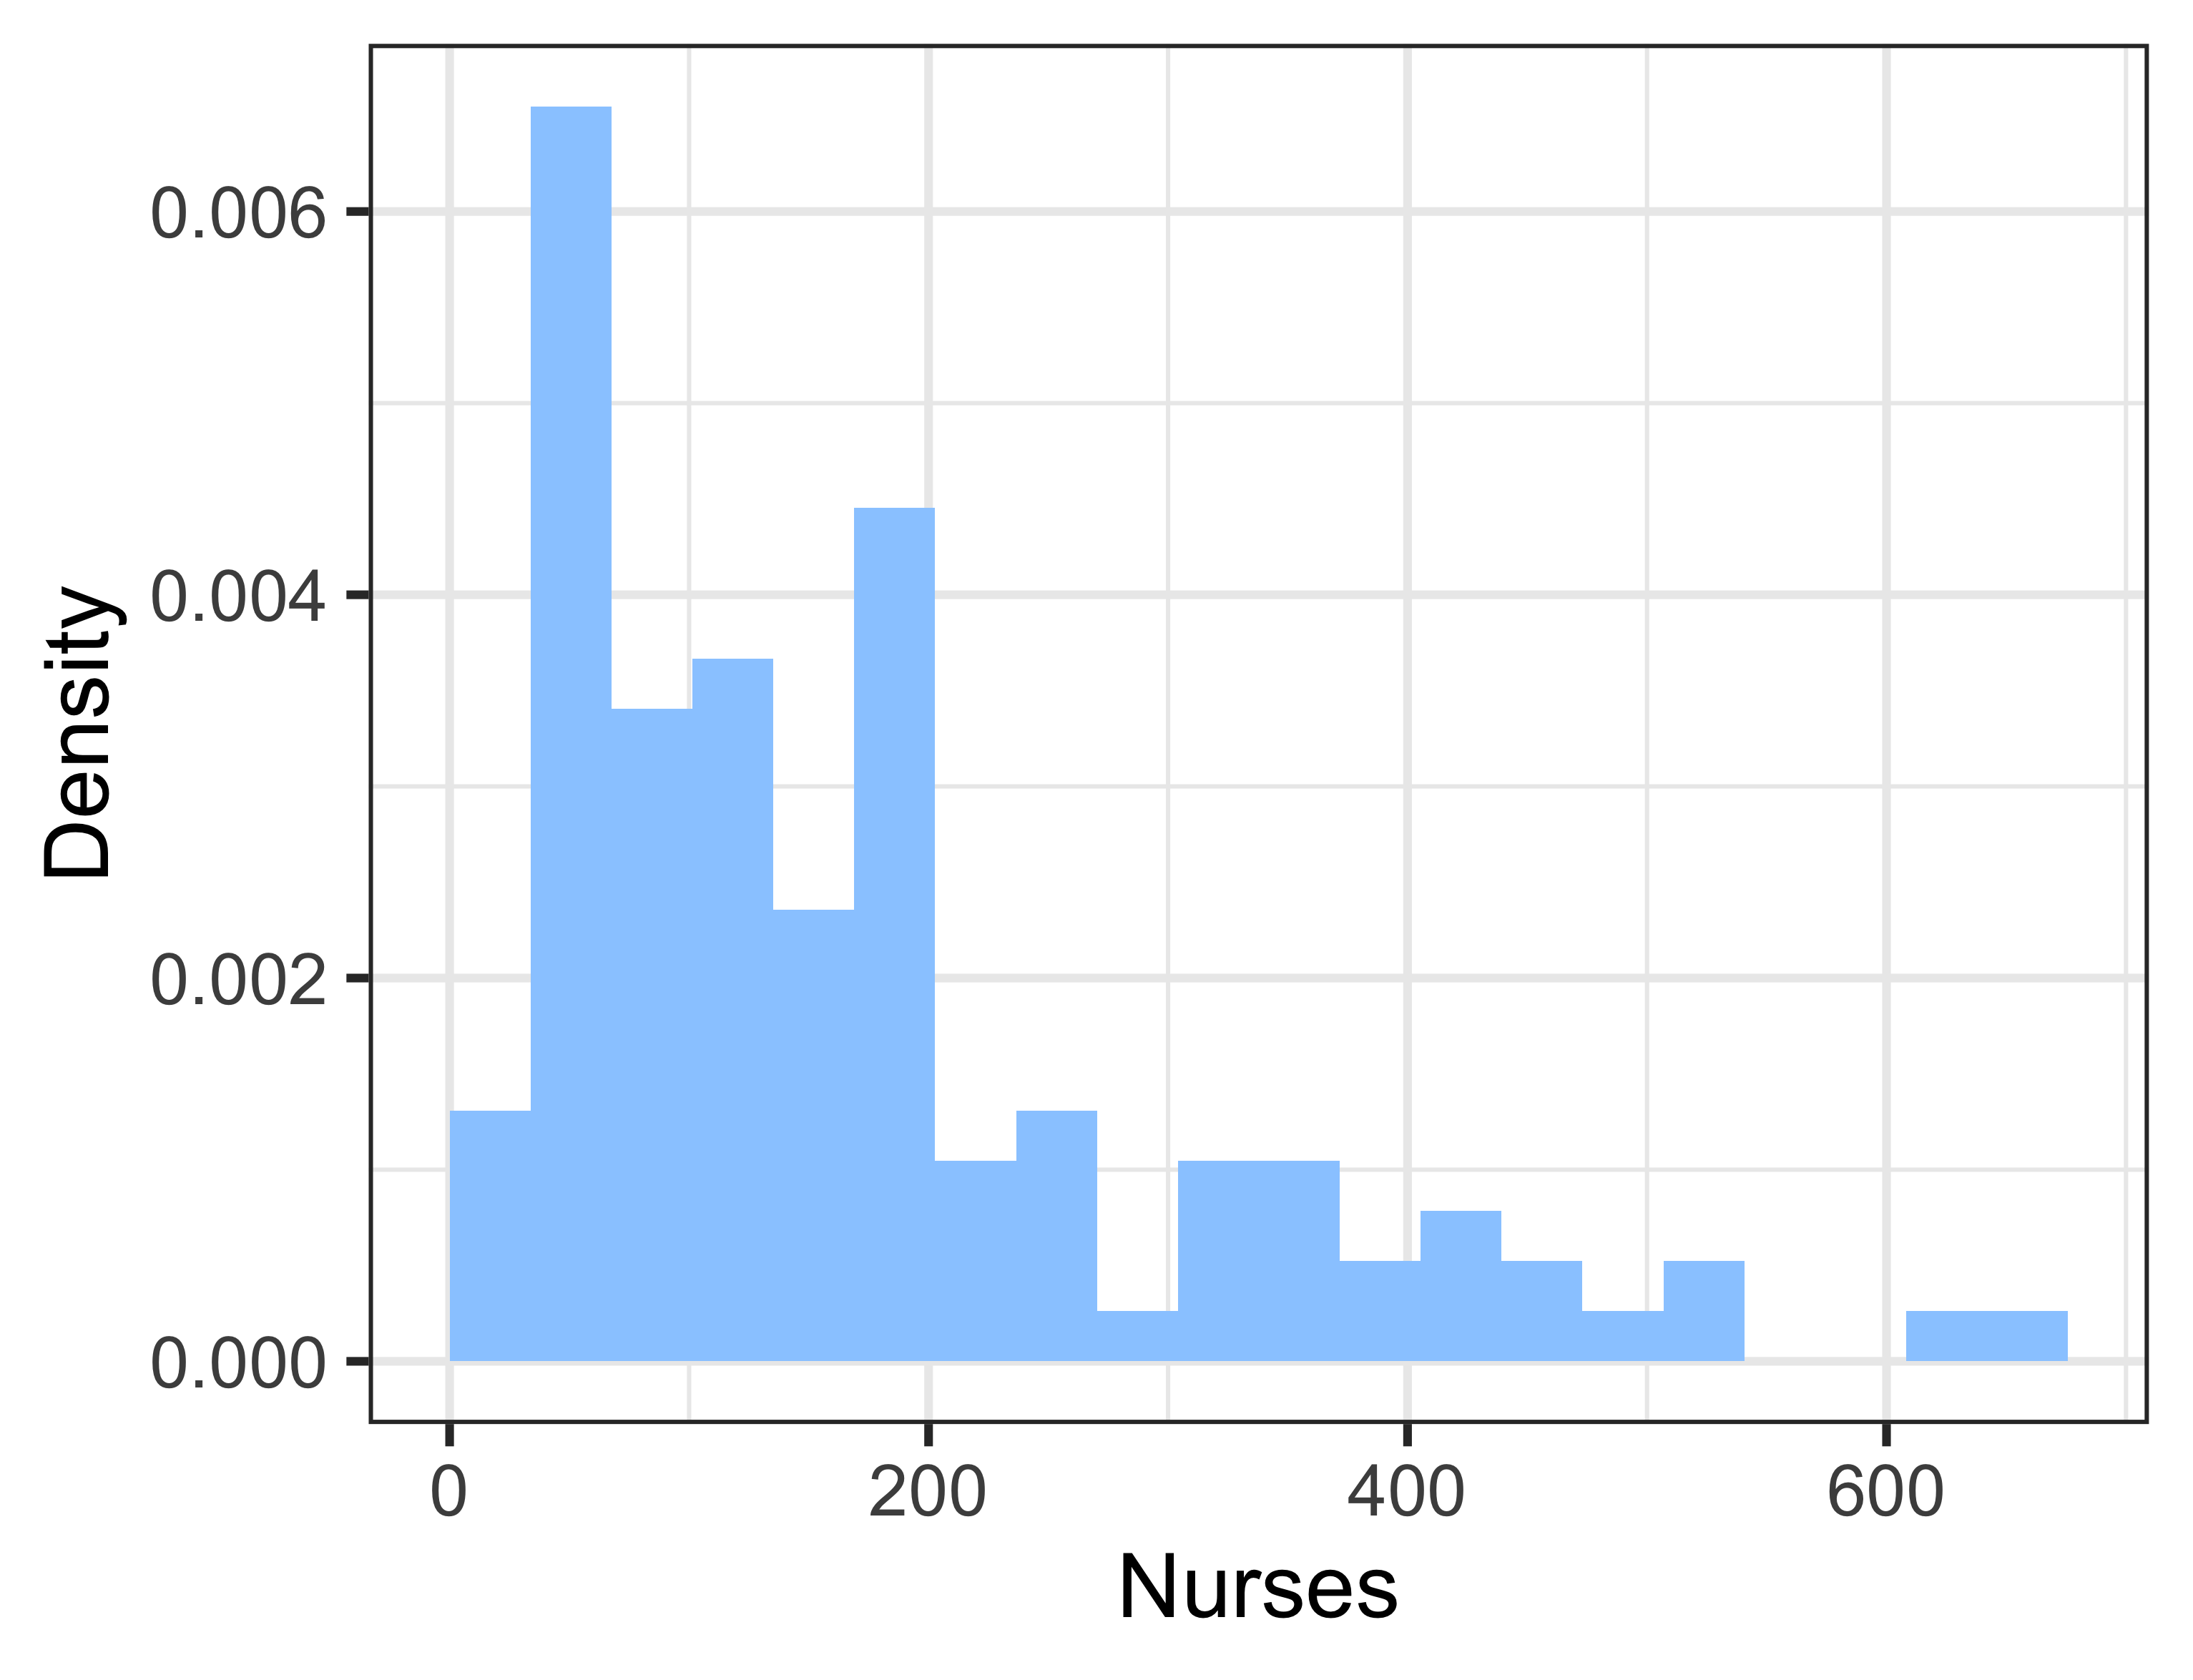
\includegraphics[width = 0.32\textwidth]{img/q01-nurses-hist-original.png}
        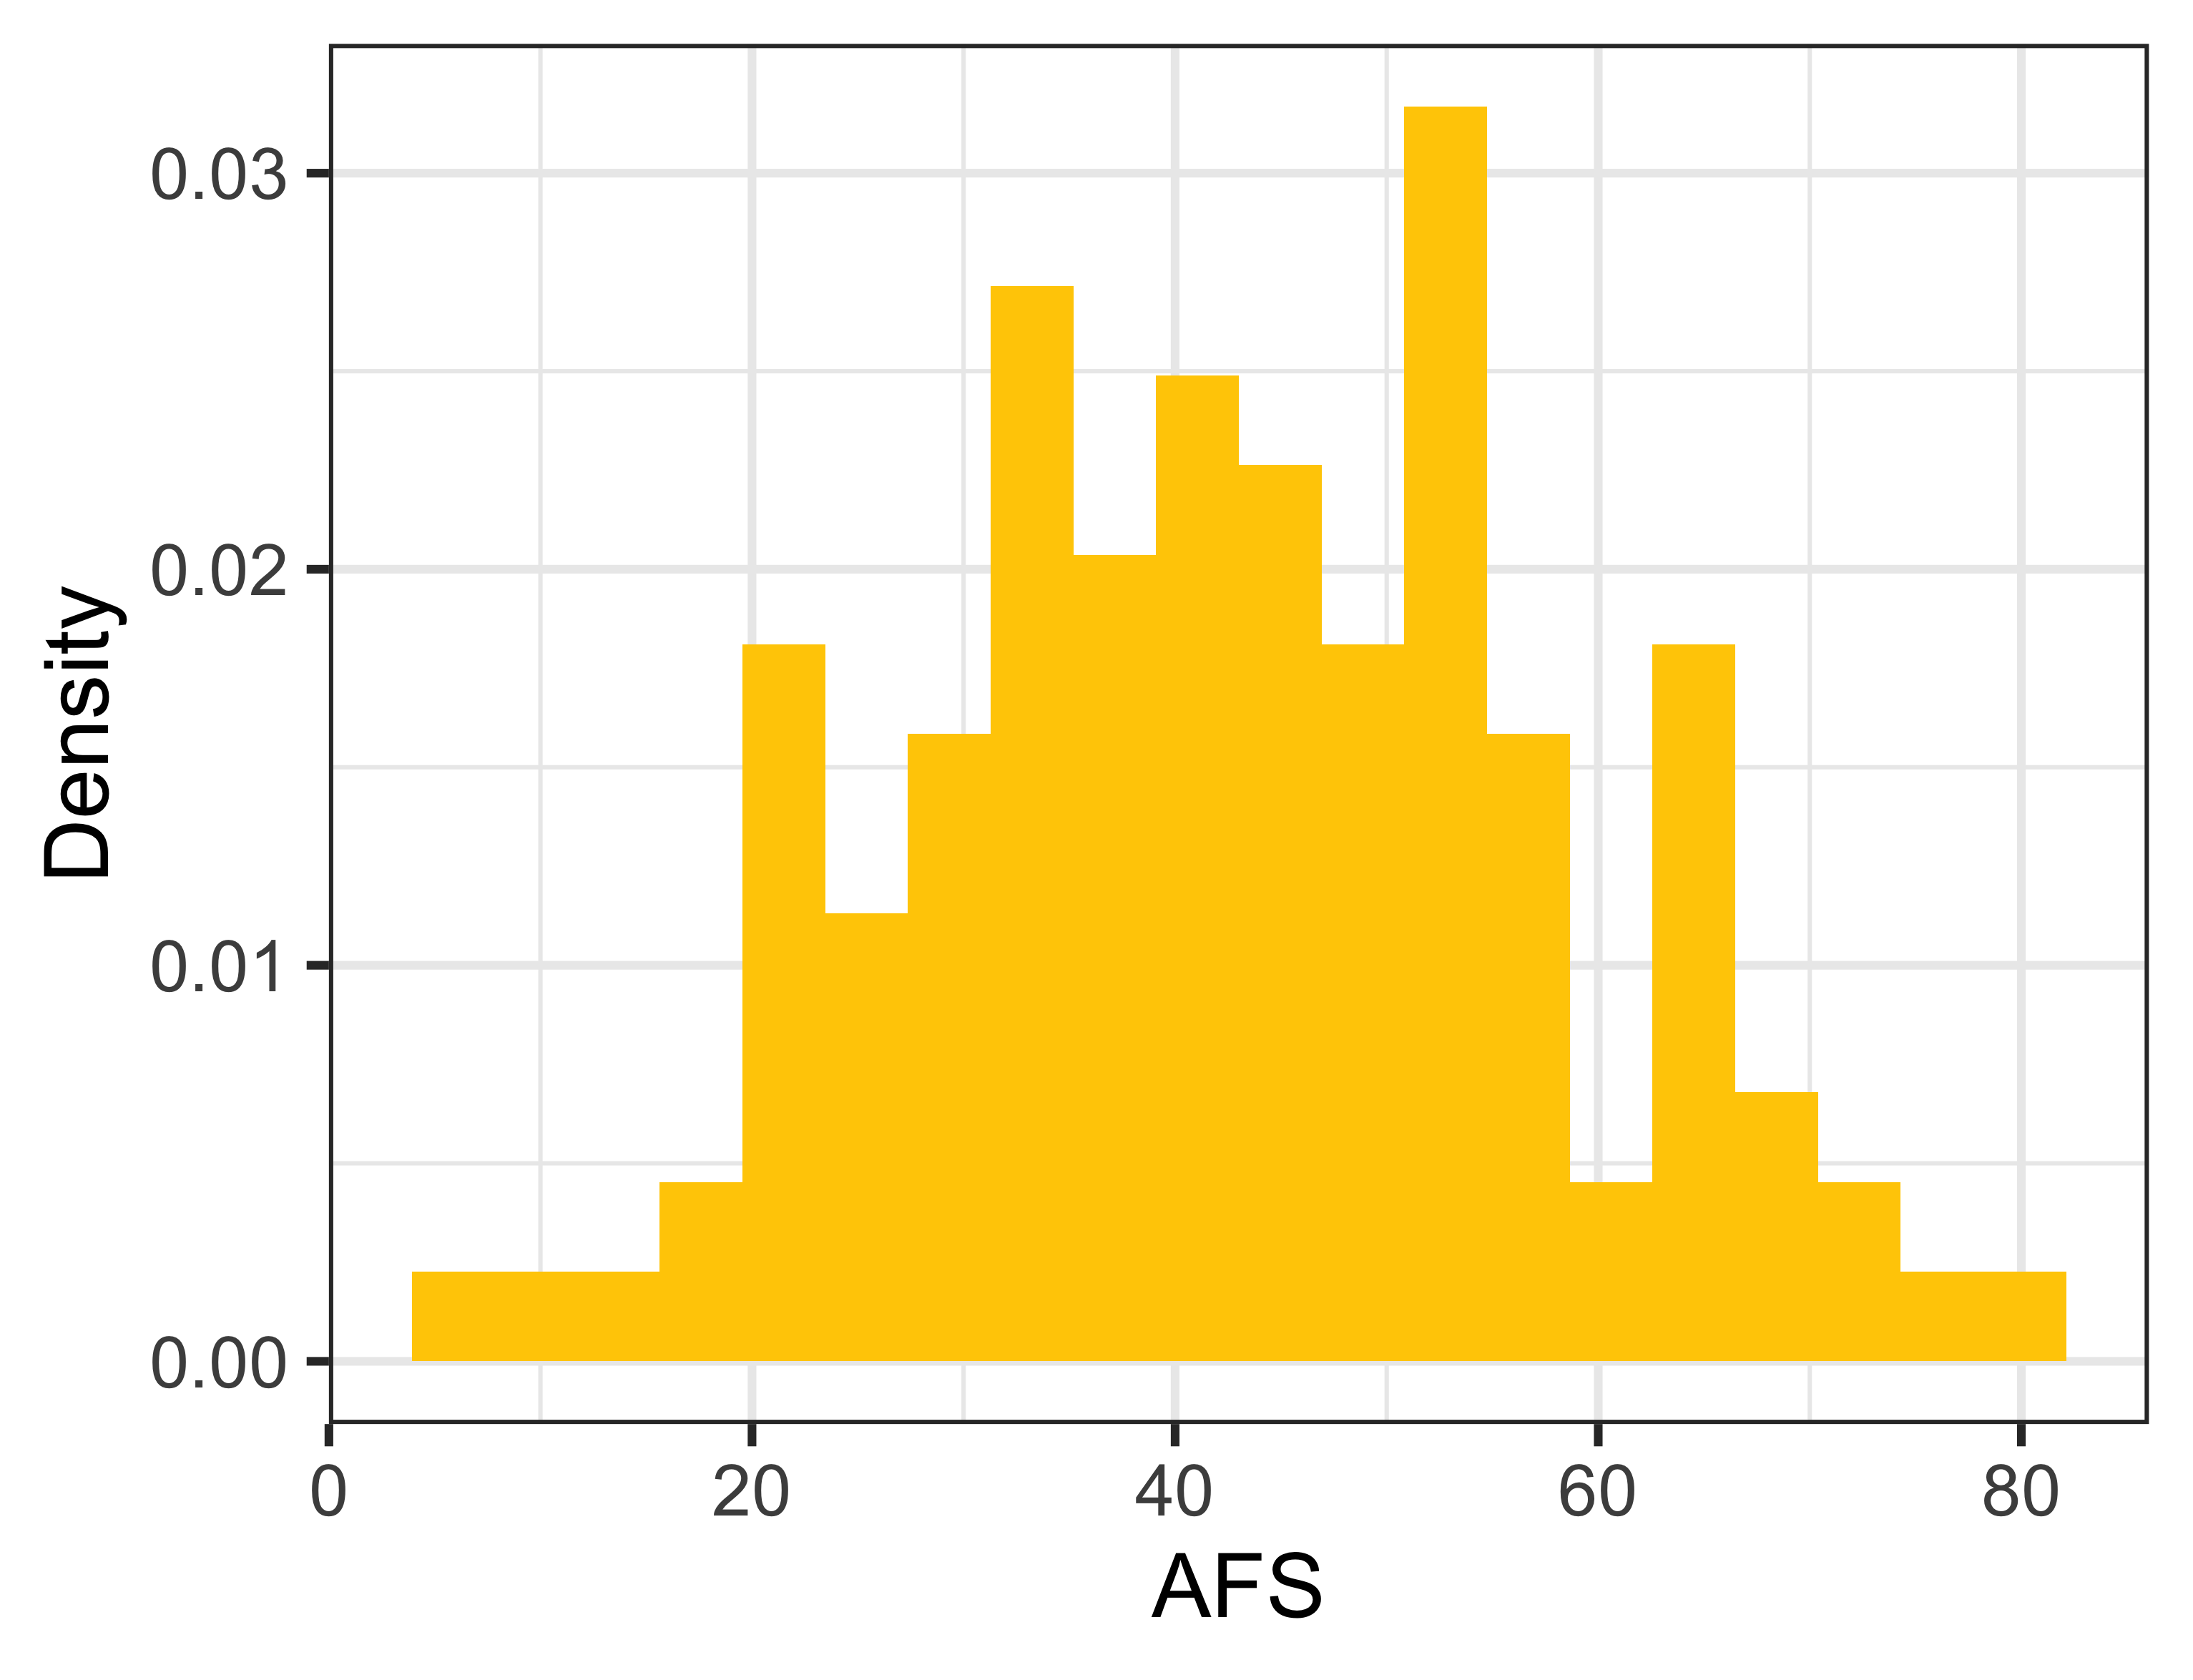
\includegraphics[width = 0.32\textwidth]{img/q01-afs-hist-original.png}
        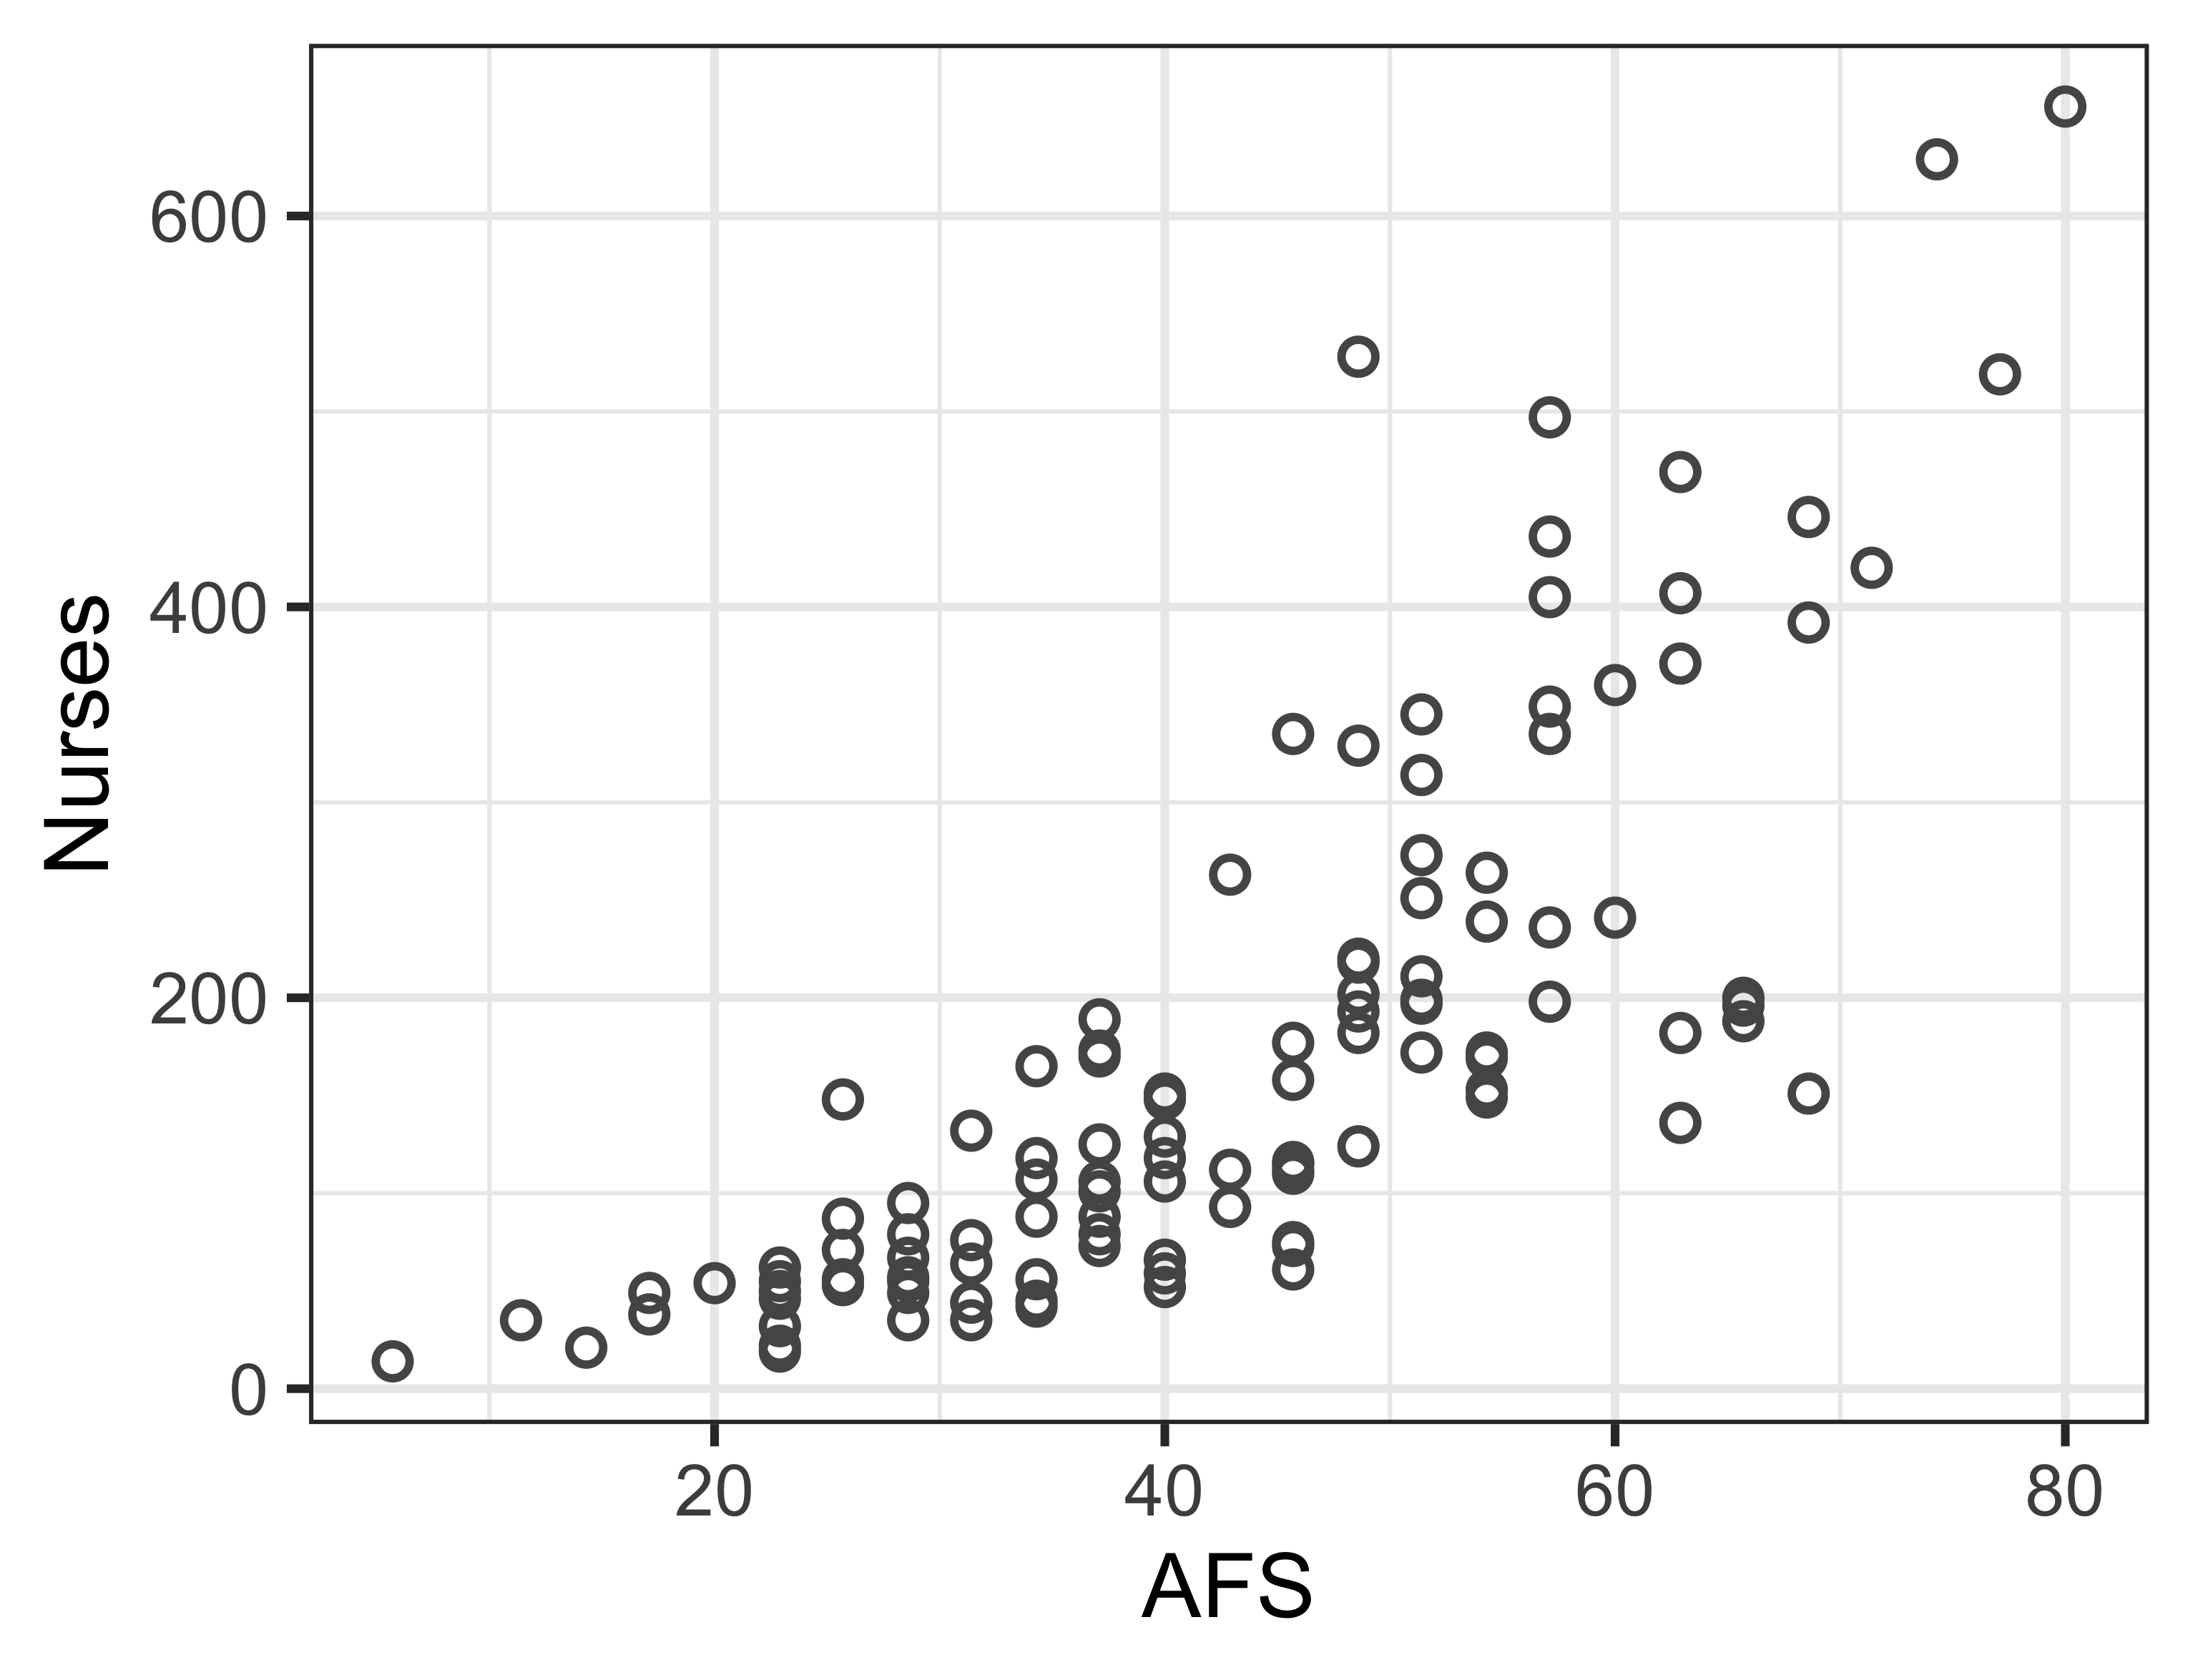
\includegraphics[width = 0.32\textwidth]{img/q01-scatterplot-blank.png}
        \caption{Histograms of \(Y\) and \(X\) and a scatterplot of \(Y\) vs. \(X\).}
        \label{q01-investigation}
    \end{figure}
    \item[(b)] The power transformation function and its scaled counterpart are defined as 
    \begin{align*}
        f_{\lambda}(Y) 
        = \begin{cases}
            % \frac{Y^{\lambda} - 1}{\lambda} & \text{if } \lambda \neq 0 \\
            \hfil Y^{\lambda} & \text{if } \lambda \neq 0 \\
            \log Y & \text{if } \lambda = 0.
        \end{cases}
        ~~~\text{and}~~~
        g_{\lambda}(Y) 
        = \begin{cases}
            % \frac{Y^{\lambda} - 1}{\lambda} & \text{if } \lambda \neq 0 \\
            (Y^{\lambda} - 1) / \lambda & \text{if } \lambda \neq 0 \\
            \hfil \log Y & \text{if } \lambda = 0.
        \end{cases}
        % g_{\lambda}^{-1}(Y) 
        % = \begin{cases}
        %     \left( 1 + \lambda Y \right)^{1 / \lambda} & \text{if } \lambda \neq 0 \\
        %      \hfil \mathrm{exp}(Y) & \text{if } \lambda = 0.
        % \end{cases}
    \end{align*}
    When transforming \(Y\), we first use the scaled power transform to fit the model \(g_{\lambda}(Y) = \beta_0 + \beta_1 X + \epsilon\) in order
    to determine an optimal value of \(\lambda\) via maximum likelihood estimation. 
    We then use \(f_{\lambda}\) to make \(Y\) closer to a normal distribution and perform any subsequent inferences. 
    % If we have our \(n\) observations (\(\mathbf{x}\),\(\mathbf{y}\)).
    In vector form, our model is \(\myg(\bm{Y}) = \beta_0 \mathbf{1} + \beta_1 \mathbf{x} + \bm{\epsilon}\), where \(\bm{\epsilon} \sim \mathrm{N}(\mathbf{0}, \sigma^2 \mathbf{I})\)
    and \(\myg(\bm{Y})\) is the transformed response (so \([\myg(\bm{Y})]_i = g_{\lambda}(Y_i)\)) for some unknown \(\lambda\). 
    % Since \(\mygfull \sim \mathrm{N}(\beta_0 \mathbf{1} + \beta_1 \mathbf{x}, \sigma^2 \mathbf{I})\), 
    It can be shown (see Appendix A) that the log-likelihood function can be expressed as a function of only \(\lambda\), 
    \begin{align*}
        m(\lambda)
        \coloneqq - \frac{n}{2} \log \left( \frac{2 \pi \mathrm{e}}{n} \right) - \frac{n}{2} \log \Big( \myg^T(\mathbf{y})(\mathbf{I} - \mathbf{H}) \myg(\mathbf{y}) \Big) + (\lambda - 1) \sum_{i=1}^n \log(y_i),
    \end{align*}
    where \(\mathbf{H} = \mathbf{X}(\mathbf{X}^T\mathbf{X})^{-1}\mathbf{X}^T\) is the hat matrix. \(m(\lambda)\) has been plotted in the left panel of Figure \ref{q01-box-cox},
    where we can see that the MLE is maximuzed at \(\lambda = 0.085\). 

    \begin{figure}[ht]
        \centering
        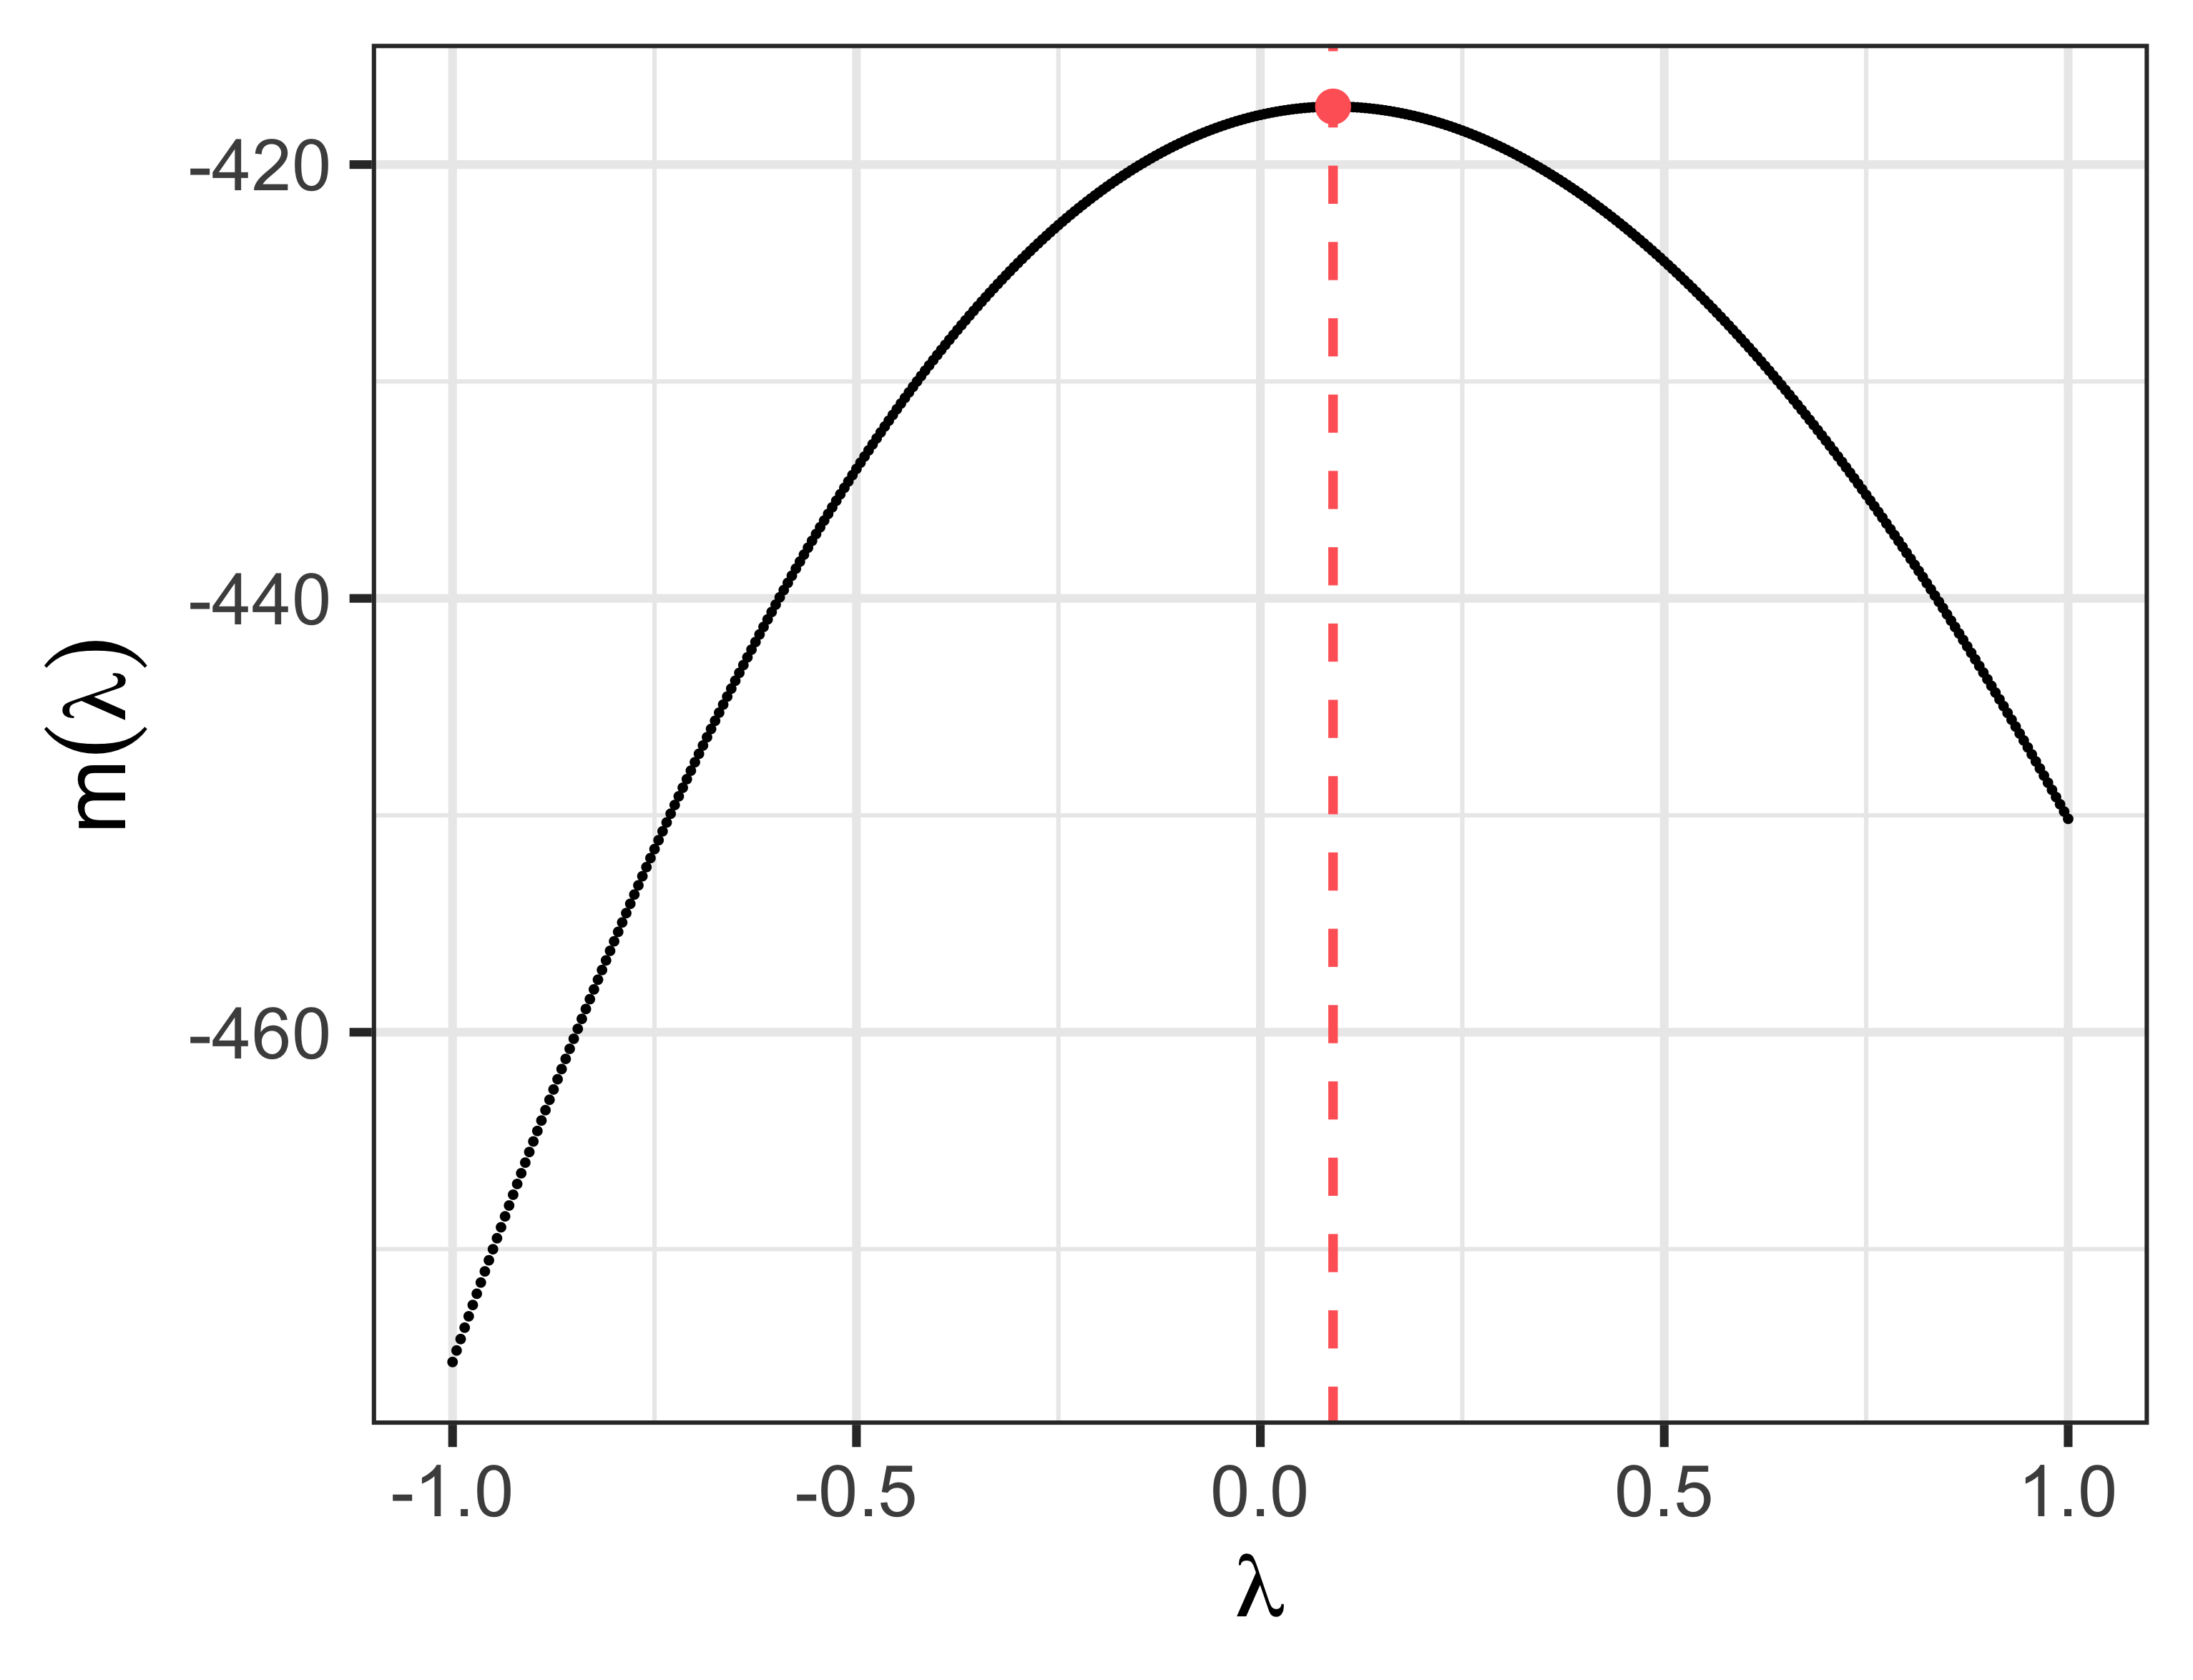
\includegraphics[width = 0.32\textwidth]{img/q01-box-cox-lambda.png}
        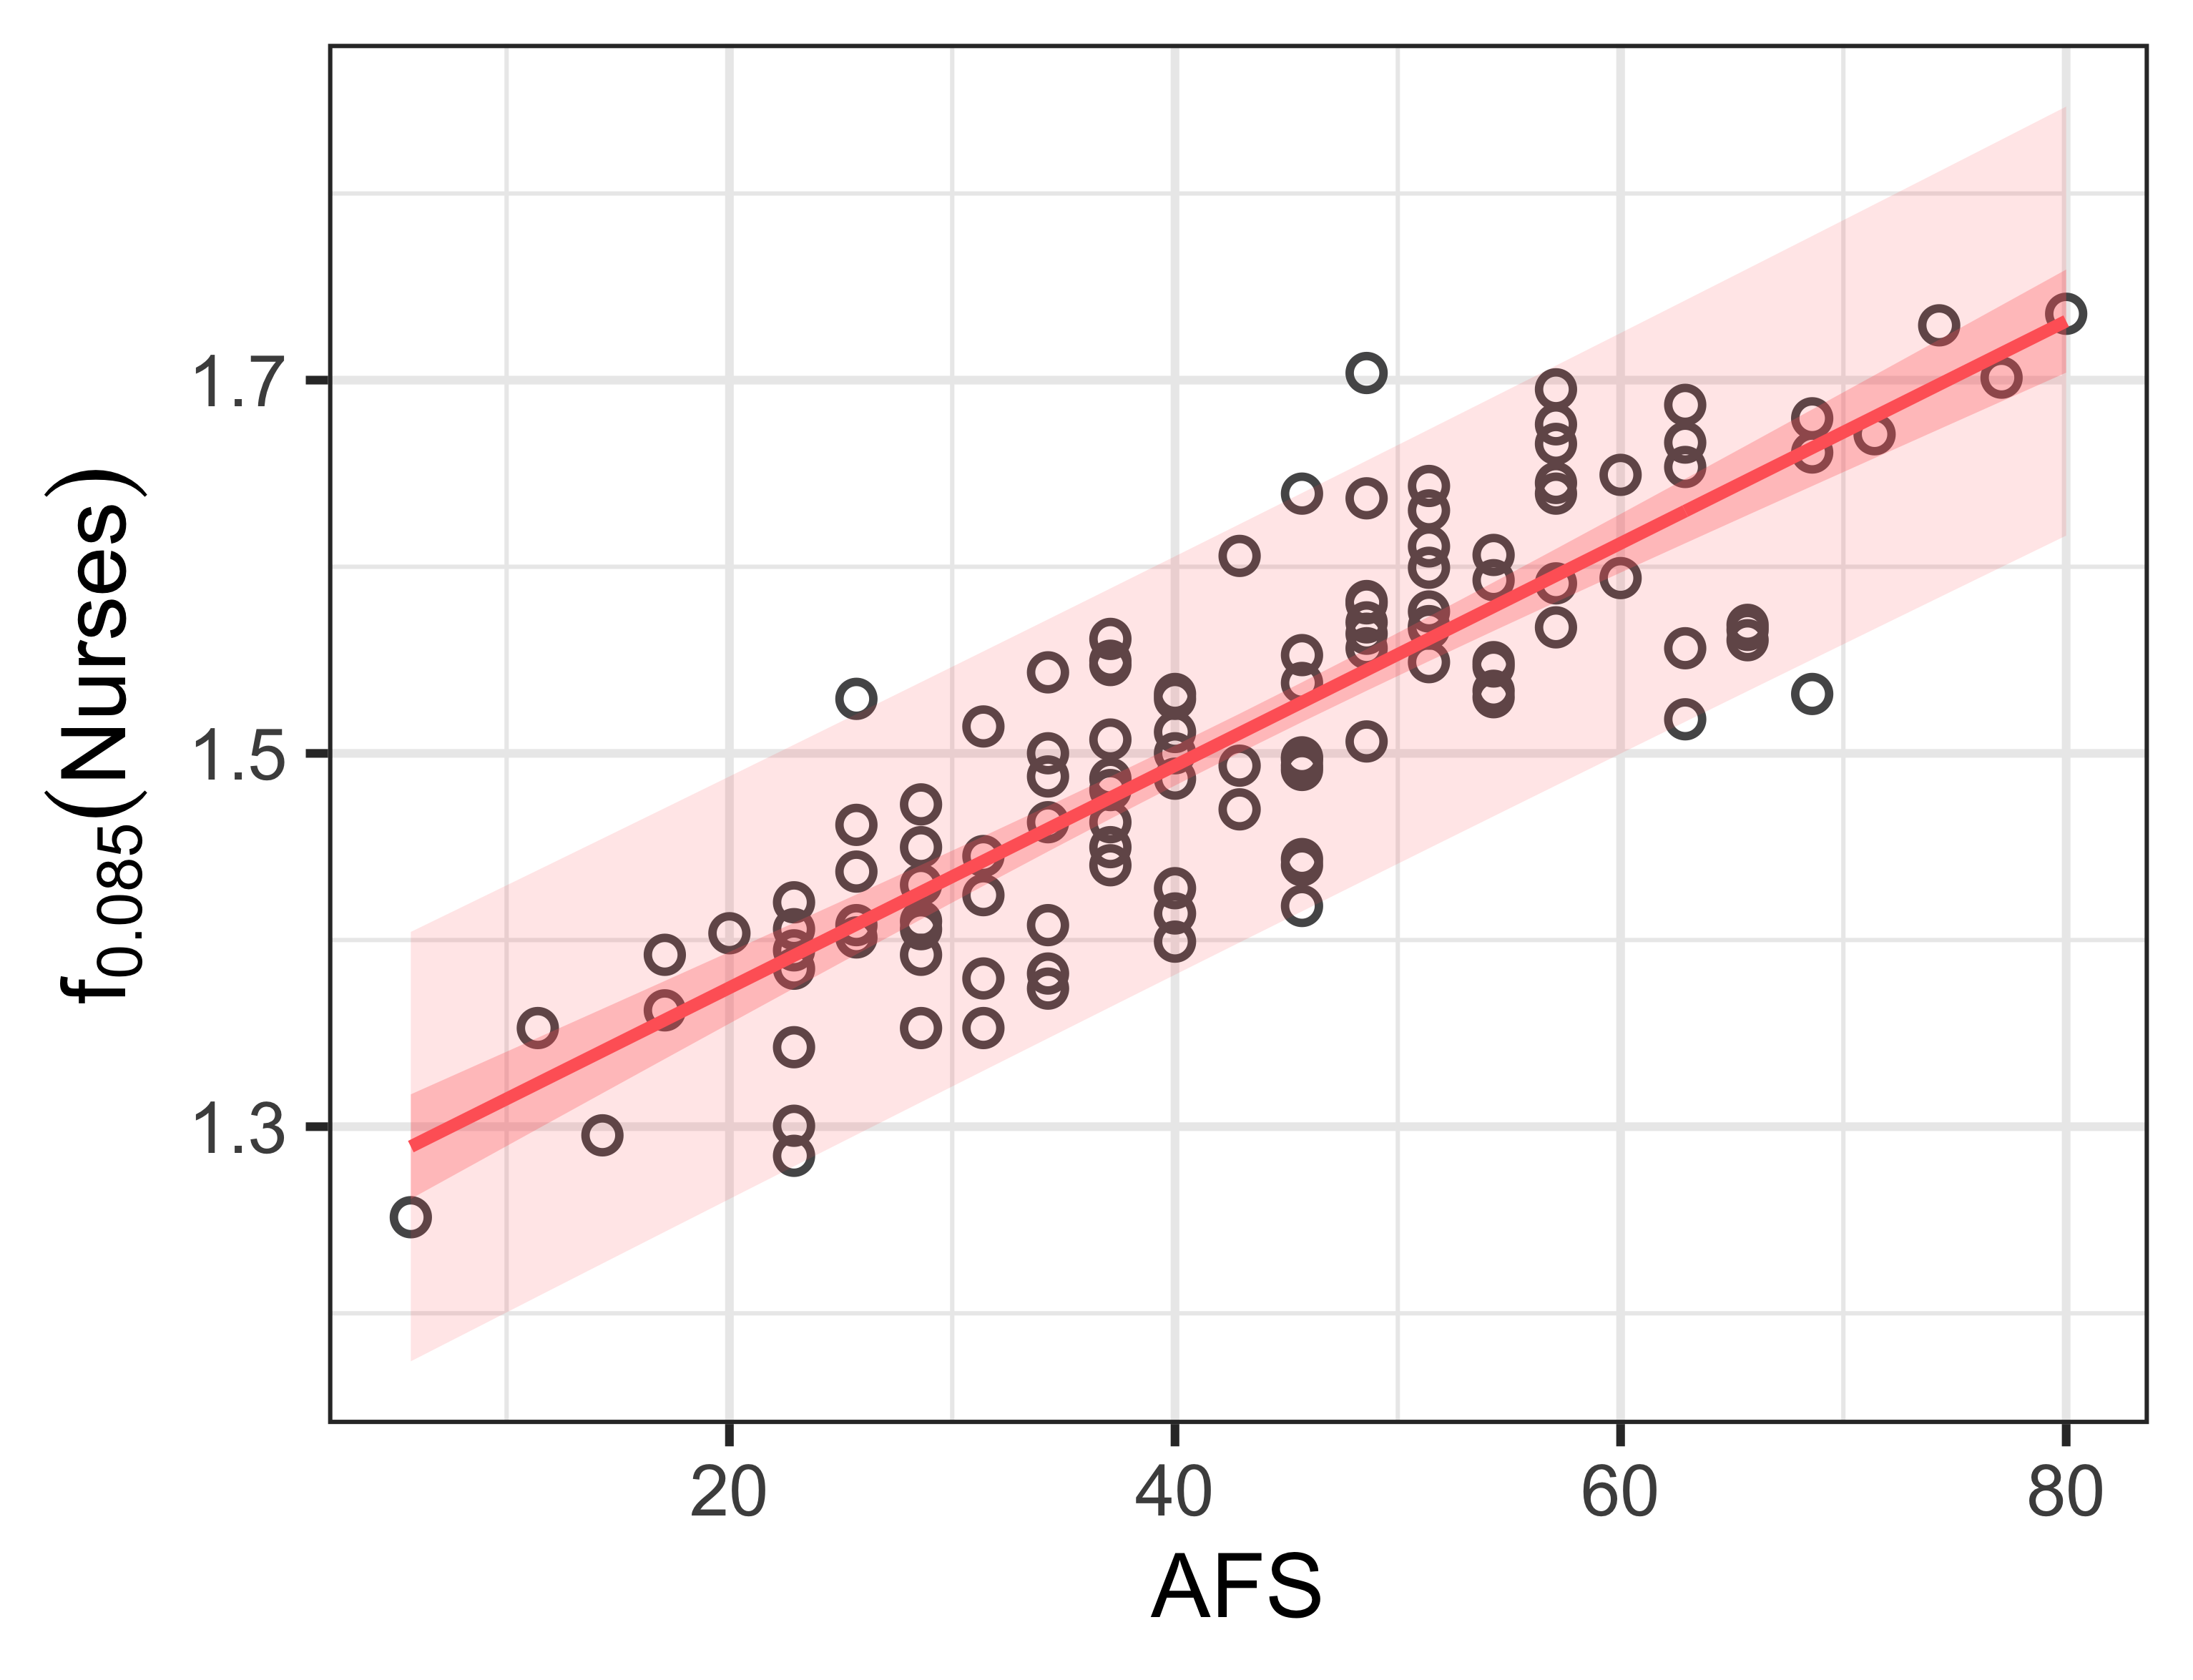
\includegraphics[width = 0.32\textwidth]{img/q01-scatterplot-power.png}
        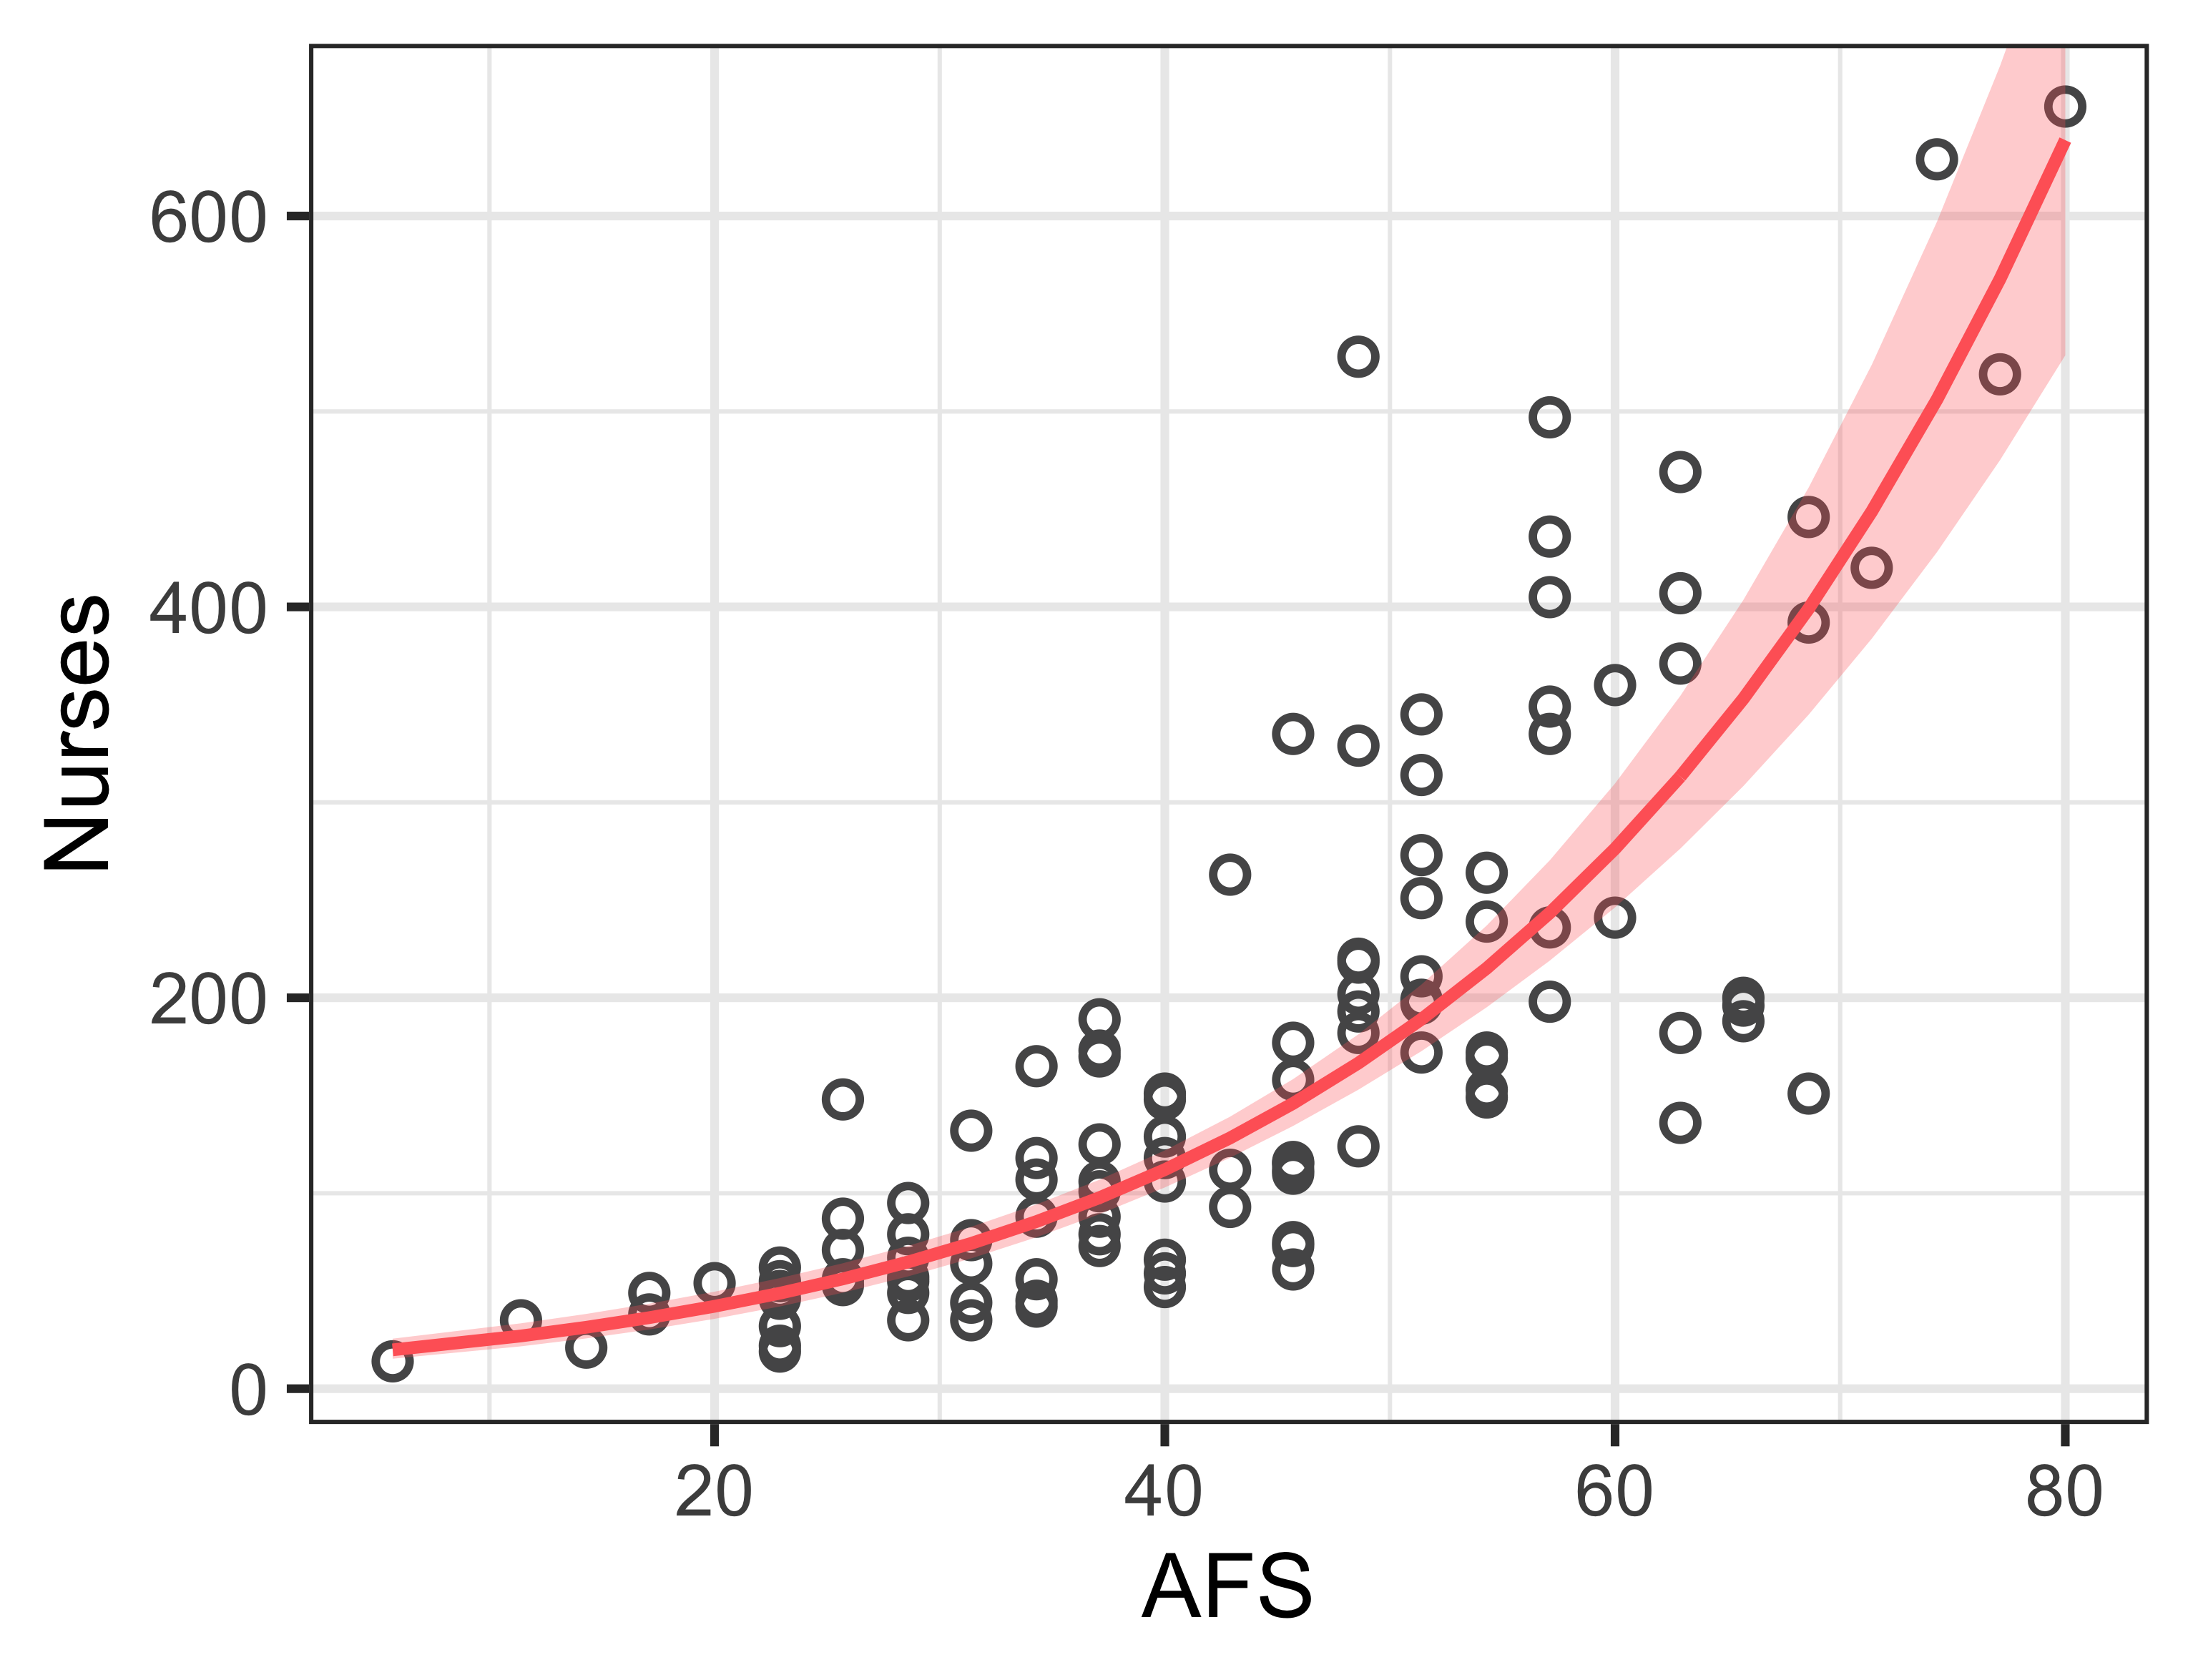
\includegraphics[width = 0.32\textwidth]{img/q01-scatterplot-nurses.png}
        \caption{Relevant plots for the power transformation of \(Y\).}
        \label{q01-box-cox}
    \end{figure}

    \item[(c)] Now that we have our optimal \(\lambda\), we will fit the model \(f_{0.085}(Y) = \beta_0 + \beta_1 X + \epsilon\). 
    We have \(\hat{\beta}_0 = 1.255\) and \(\hat{\beta}_1 = 0.005953\). A plot of this model, along with a \(95\)\%{} confidence interval,
    has been printed in the middle panel of Figure \ref{q01-box-cox}. This means that when \(X\) increases by 1 unit, \(f_{0.085}(Y)\)
    is expected to increase by \(0.005953\) units. We can also make inferences about \(Y\) itself; we have 
    \(Y = f_{0.085}^{-1}(\hat{\beta}_0 + \hat{\beta}_1 X) = \big(1.255 + 0.005953 X)^{1 / 0.085}\). A plot of this model has been printed in 
    the right panel of Figure \ref{q01-box-cox}. 
    % This means that when \(X\) increases by one unit, \(Y\) is expected to increase by \(\big(1.255 + 0.005953)^{1 / 0.085} = 15.3\) units. 
    We must keep in mind that this model is non-linear, so it's expected rate of change will depend on the value of \(X\). 

    \item[(d)] Both diagnostic plots can be found in Figure \ref{q01-diagnostics}, and the data seems to confirm the model assumptions very well.
    \begin{figure}[ht]
        \centering
        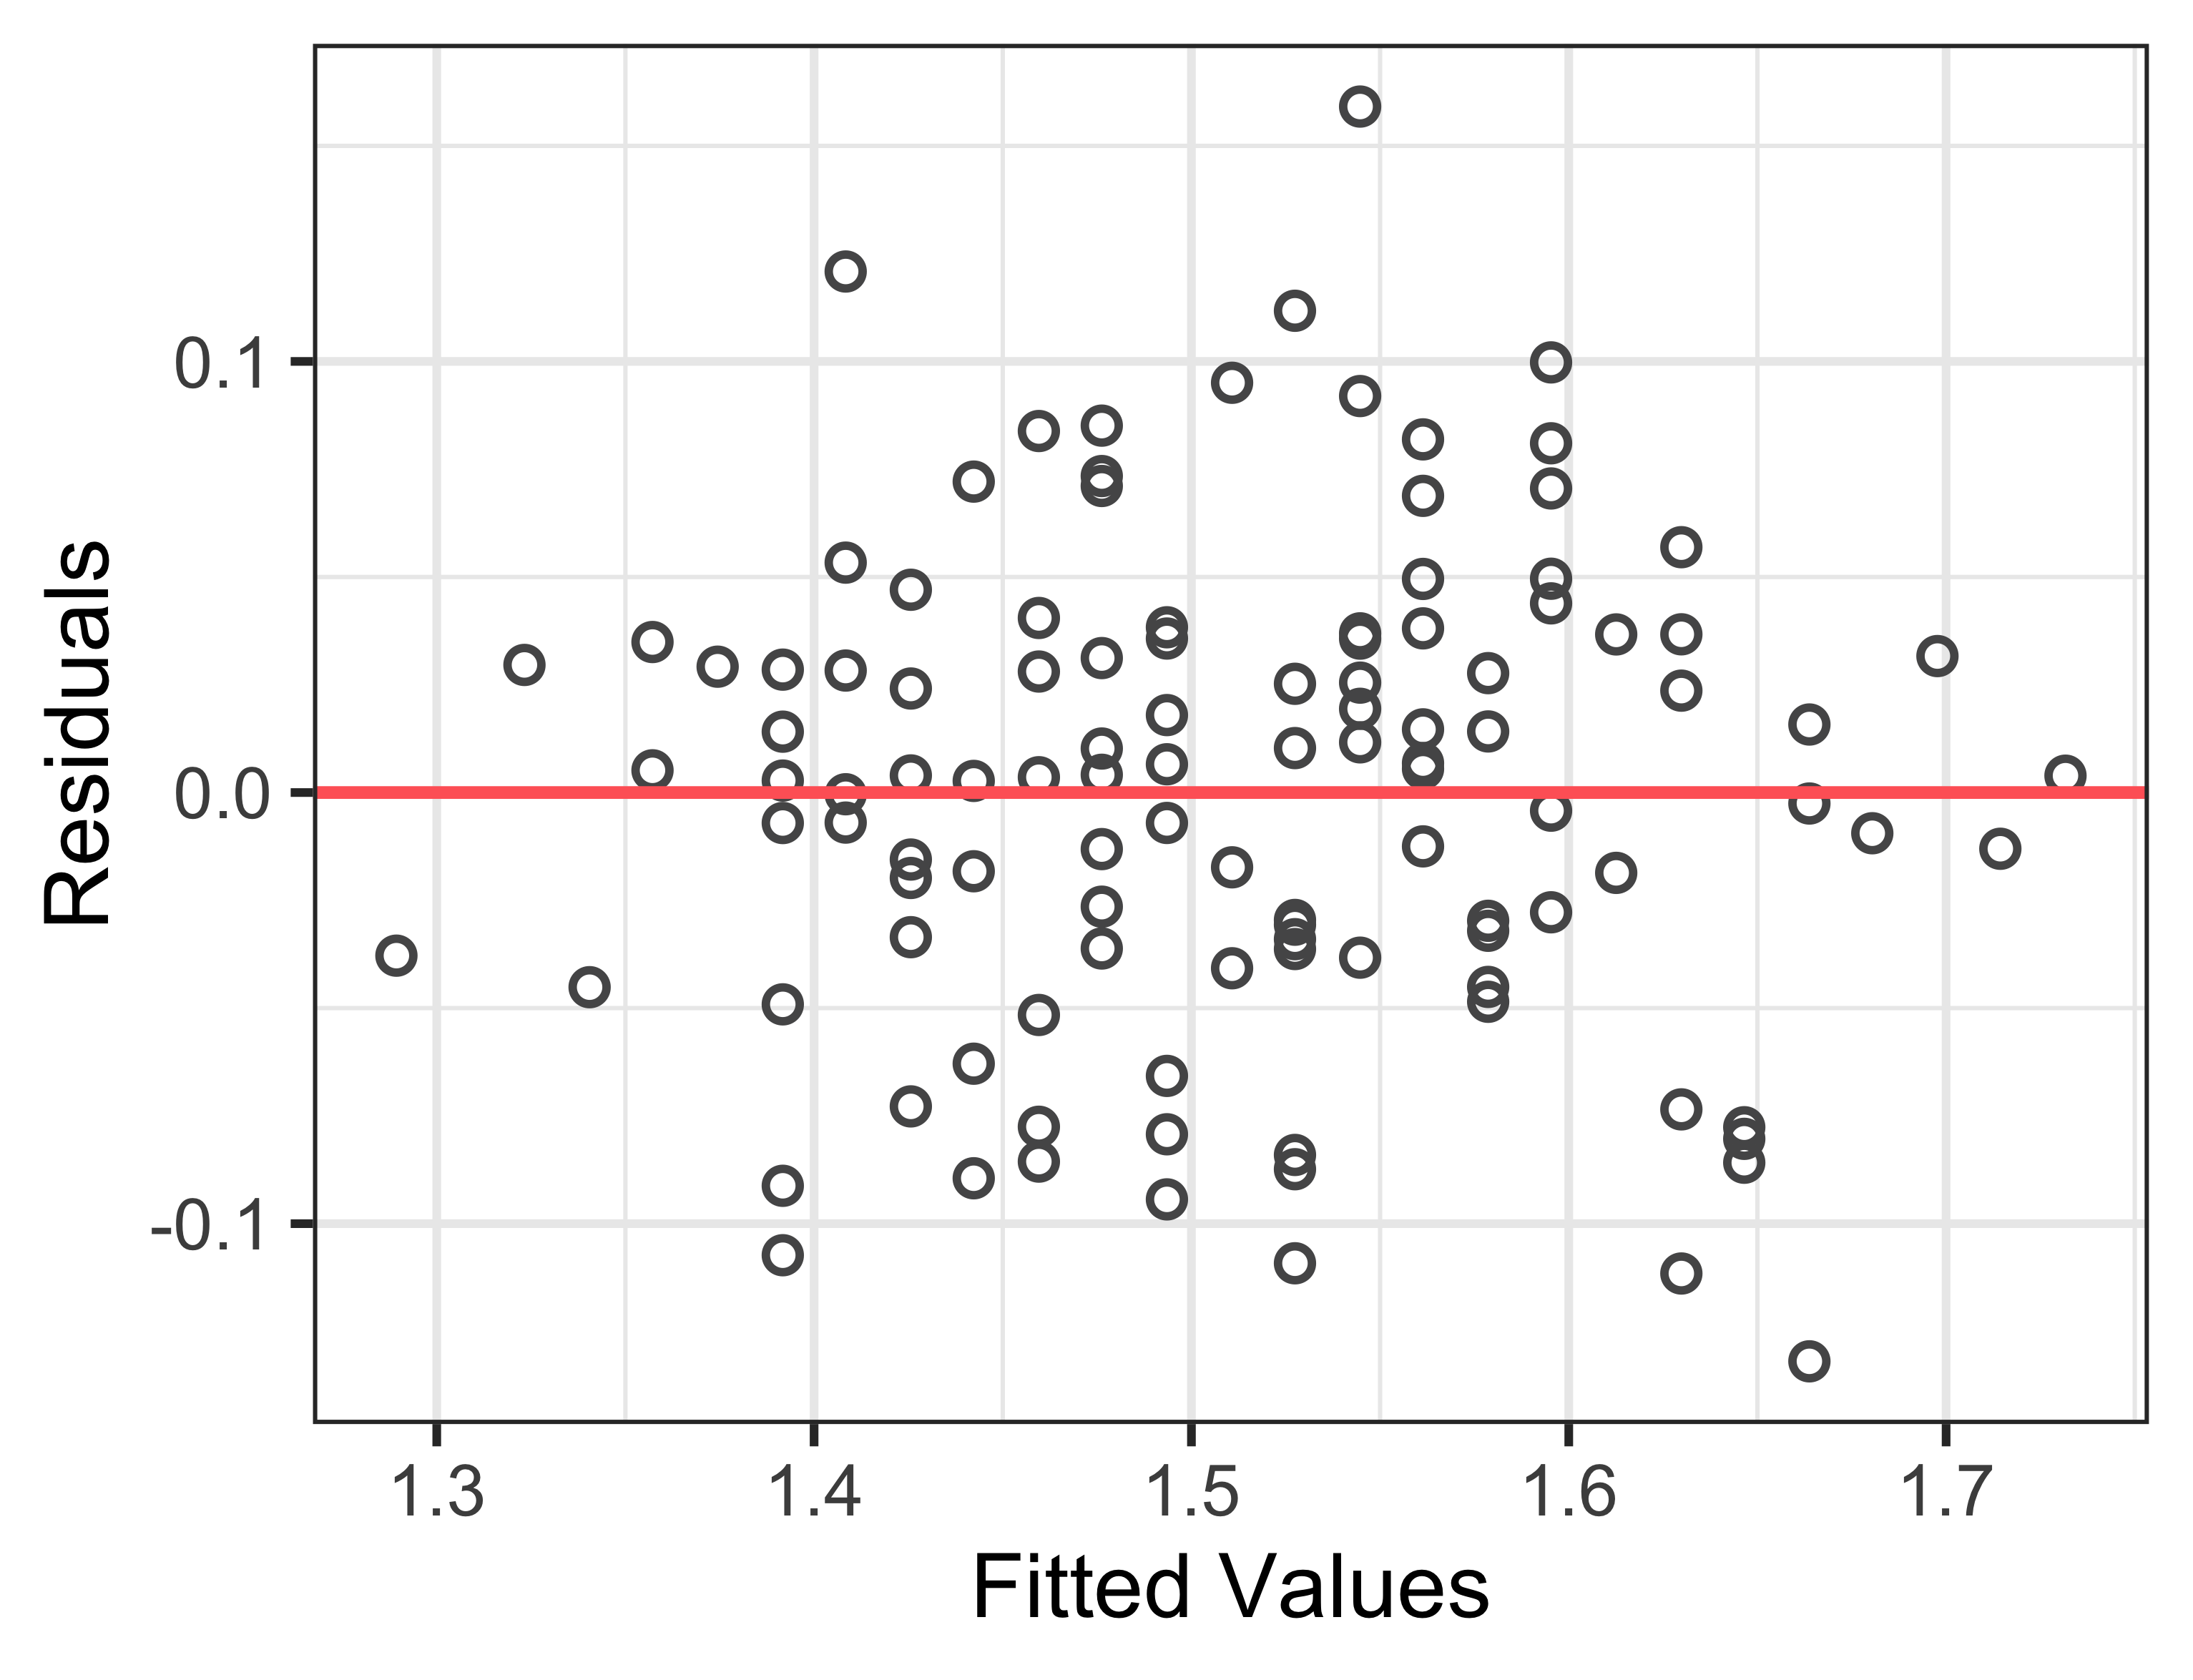
\includegraphics[width = 0.4\textwidth]{img/q01-diagnostic-residuals.png}
        \quad
        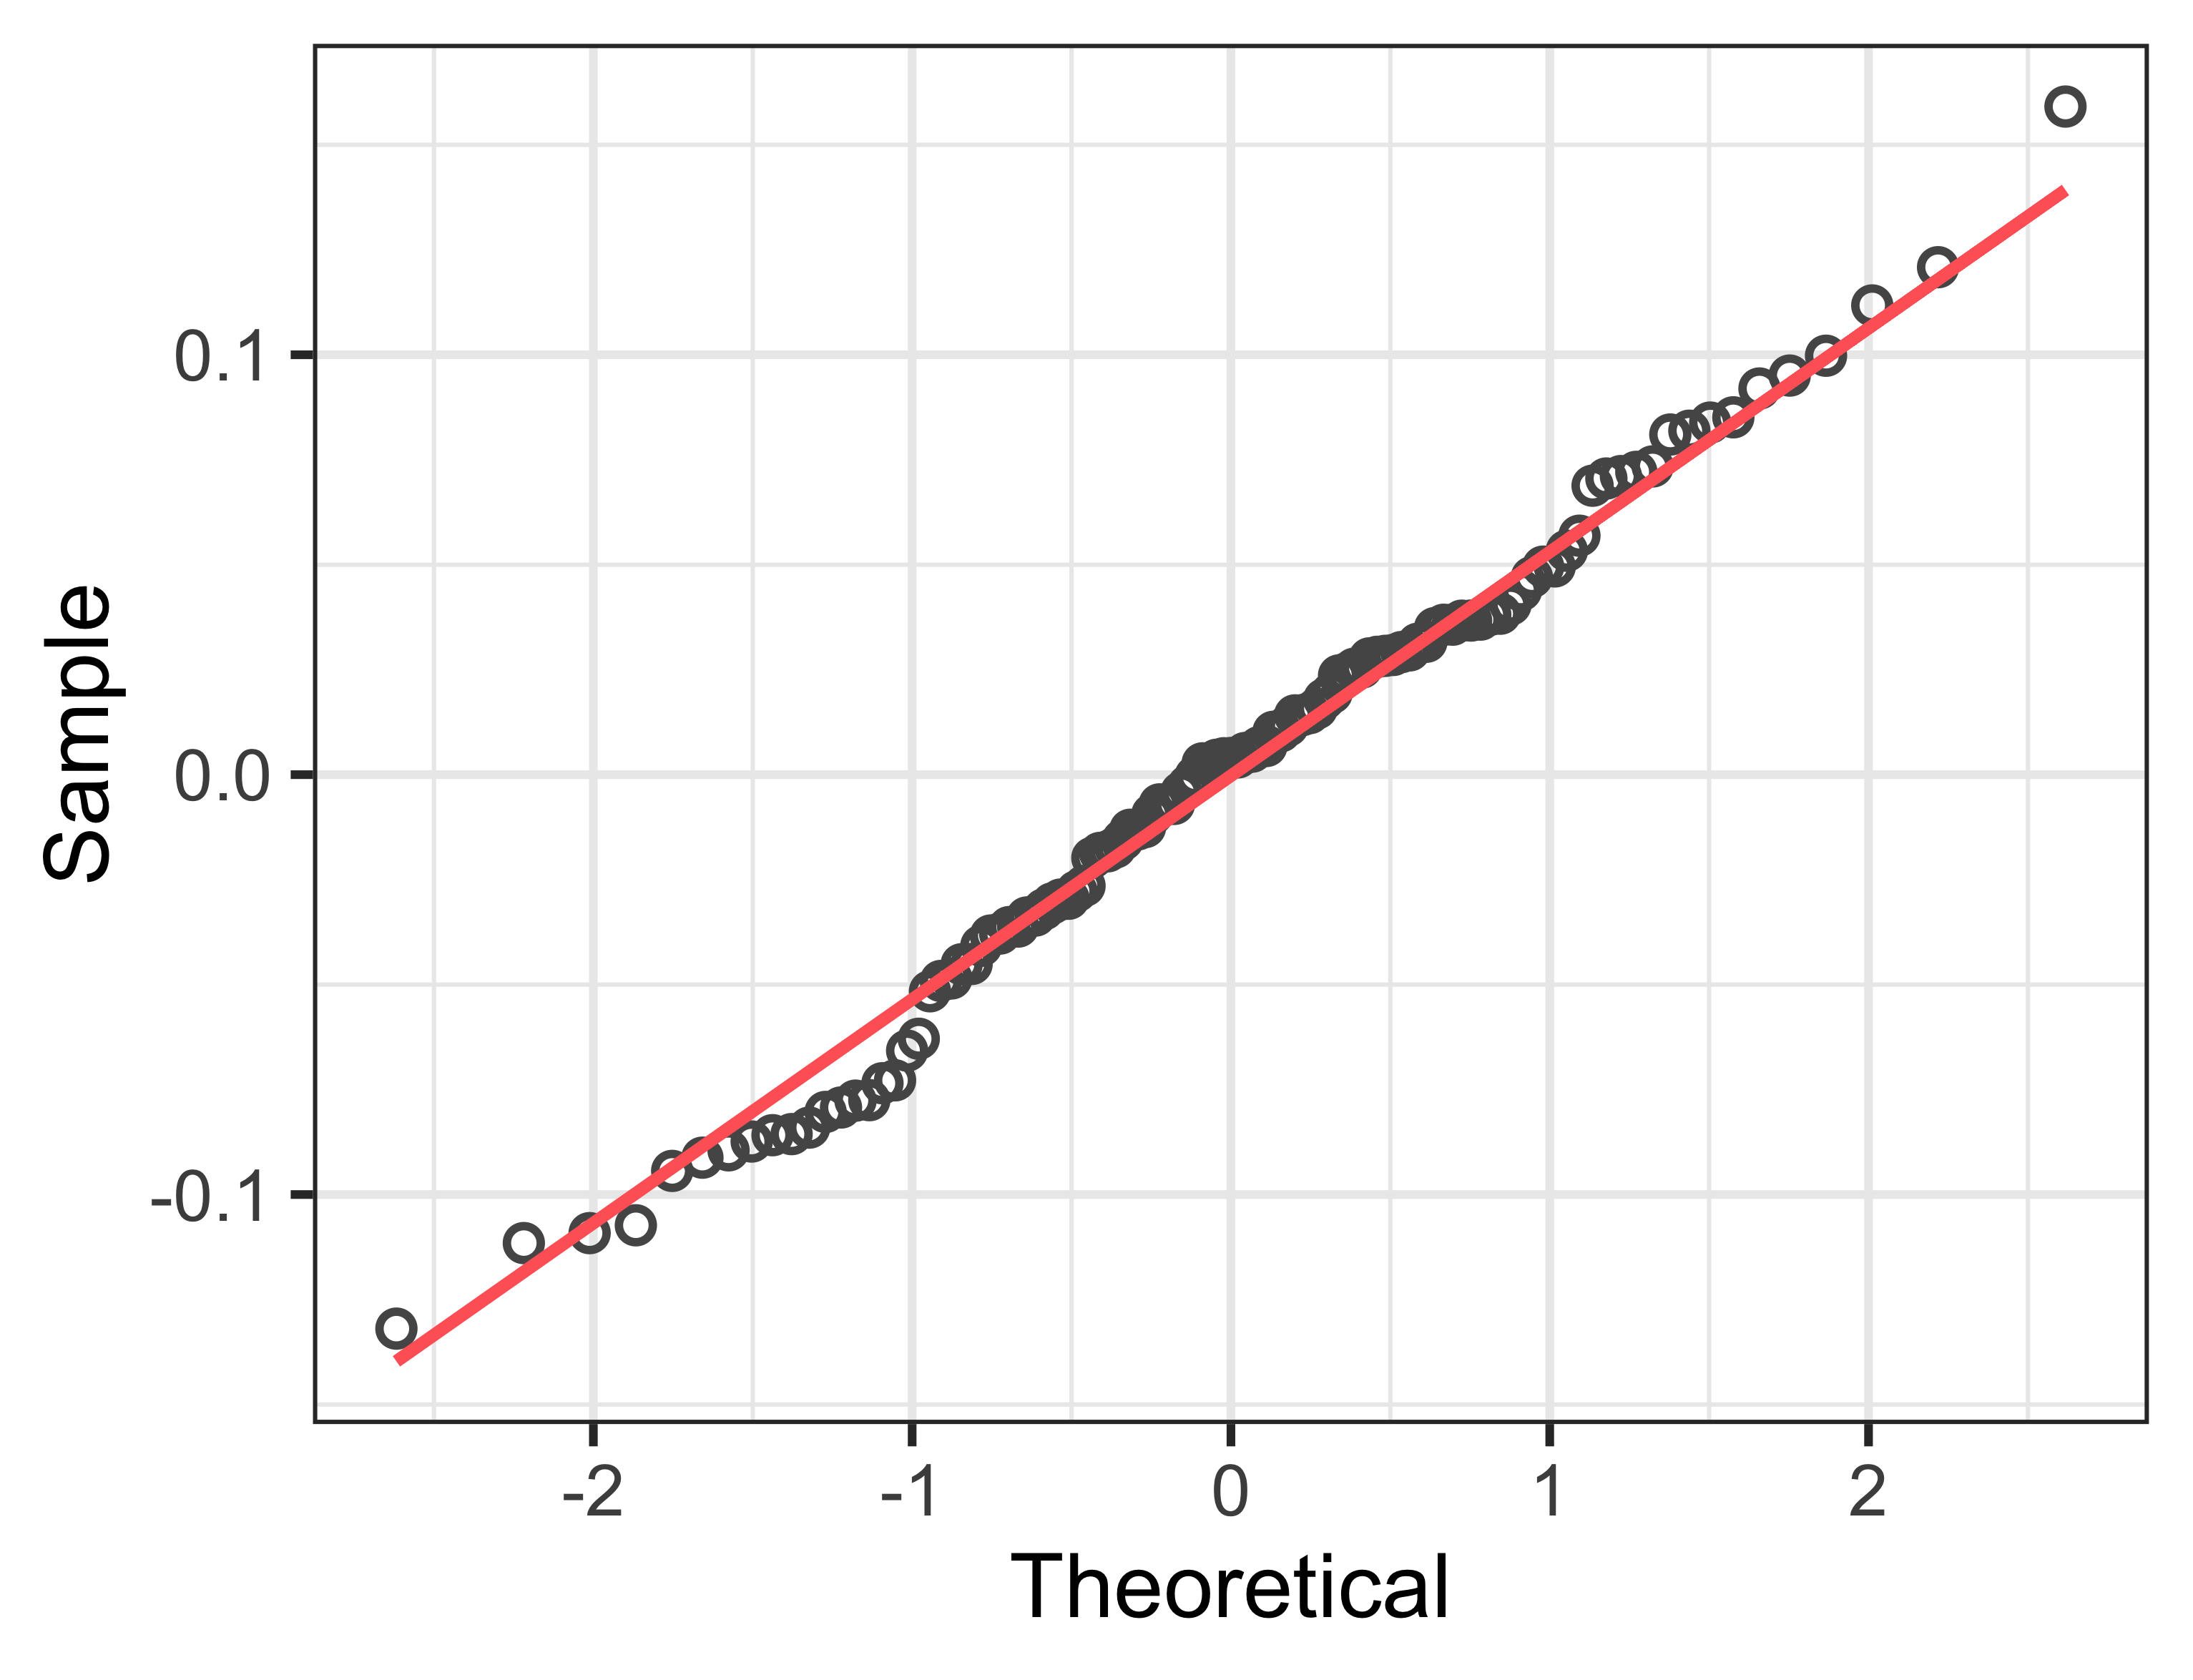
\includegraphics[width = 0.4\textwidth]{img/q01-diagnostic-qqplot.png}
        \caption{Diagnostic plots for the power transformation model.}
        \label{q01-diagnostics}
    \end{figure}

    \item[(e)] We cannot conduct an \(F\)-test on the two models. This is because both models have the same number of parameters that need to be estimated,
    meaning they both have the same number of degrees of freedom. 

    \item[(f)] In order to find a prediction interval for \(Y\), we can first find a prediction interval for \(f_{0.085}(Y)\) and then apply \(f_{0.085}^{-1}\)
    to both ends of the interval. The prediction intervals for when \(X = 30\) and \(X = 60\) have been printed in Table \ref{q01-prediction-intervals}. 
    For reference, the prediction intervals at these observations for the linear model \(Y = \beta_0 + \beta_1 + \epsilon\) have also been printed. 
    The prediction intervals for the power model can also be seen in the middel and right plots of Figure \ref{q01-box-cox}. 
    For starters, the width of the intervals for the power model drastically increases as \(X\) increases, while the increase for the linear model is negligible. 
    When \(X = 30\), the confidence interval for the power model is significantly narrower than the linear function, but when \(X = 60\), the opposite is true. 
    % When \(X = 30\), using the power model we are \(95\)\%{} sure that the 
    That is, when \(X = 30\) we are confident that the next observation will lie in a smaller interval using the power model, but when \(X = 60\), the linear model 
    gives us the smaller region. Depending on the value of \(X\), I would use the better of the two models. 

    \begin{table}[ht]
        \def\arraystretch{1.25}
        \centering
        \begin{tabular}{|l|cccc|cccc|}
            \hline%
            &\multicolumn{4}{|c|}{\(X = 30\)} & \multicolumn{4}{|c|}{\(X = 60\)}\\
            \hline%
            Model & \(\hat{Y}\) & Lower & Upper & \(\Delta\mathcal{I}\) & \(\hat{Y}\) & Lower & Upper & \(\Delta\mathcal{I}\)\\
            \hline%
            Linear & 74.612 & \(-89.781\) & 239.004 & 328.785 & 297.769 & 133.036 & 462.503 & 329.467 \\
            Power  & 69.448 & 26.573      & 168.796 & 142.223 & 276.313 & 117.843 & 611.638 & 493.795 \\
            \hline%
        \end{tabular}
        \caption{Comparing the prediction intervals of the linear model against the power model.}
        \label{q01-prediction-intervals}
    \end{table}
\end{itemize}

\newcommand{\gmat}{\mathbf{G}_{\bm{\lambda}}}
\newcommand{\myga}{\mathbf{g}_{\theta}}
\newcommand{\mygp}[1]{\mathbf{g}_{\lambda}(#1)}
\newcommand{\mygap}[1]{\mathbf{g}_{\theta}(#1)}
%' ============================================================================================================================================================
\section{Question 2} \noindent
\mycolaba{None}
\begin{itemize}
    \item[(a)] We are now applying the scaled power function to both the response and each of the predictors of interest. Let \(Y\) be the length of stay and 
    \(Z_1, \ldots, Z_8\) be average age of patients, infection risk, cultering ratio, X-ray ratio, number of beds, average daily census, number of nurses, and 
    available facilities and services, respectively. To find optimal parameters for transformation, we will fit the model 
    \begin{align}
        g_{\theta}(Y)
        = \beta_0 + \sum_{i = 1}^8 \beta_i \cdot g_{\lambda_{i}}(Z_i) + \epsilon,
        \label{model-senic-both}
    \end{align}
    where \(\epsilon \sim \mathrm{N}(0, \sigma^2)\), and use MLE to find the optimal values of \(\theta\) and \(\bm{\lambda} = (\lambda_1, \ldots, \lambda_8)^T\).
    The values suggested by the initial question are \(\theta_0 = -1\) and \(\bm{\lambda}_0 = (1,1,0,1,0,0,0,1)^T\).
    Using vector notation, our model can be written as \(\mygap{\bm{Y}} = \gmat \bm{\beta} + \bm{\epsilon}\), where 
    \(\gmat = \begin{bmatrix}
        \mathbf{1} & \mathbf{g}_{\lambda_1}(\mathbf{z}_1) & \mathbf{g}_{\lambda_8}(\mathbf{z}_8)
    \end{bmatrix}\)
    is the matrix of predictors transformed by \(g_{\lambda}\). It can be shown (see Appendix B) that the log-likelihood can be expressed as a function of only the
    unknown parameters \(\theta\) and \(\bm{\lambda}\), 
    \begin{align*}
        m(\theta, \bm{\lambda})
        \coloneqq - \frac{n}{2} \log \left( \frac{2 \pi \mathrm{e}}{n} \right) - \frac{n}{2} \log \Big( \myga^T(\mathbf{y})(\mathbf{I} - \mathbf{H}_{\bm{\lambda}}) \myga(\mathbf{y}) \Big) + (\theta - 1) \sum_{i=1}^n \log(y_i),
    \end{align*}
    where \(\mathbf{H}_{\bm{\lambda}} = \gmat (\gmat^T \gmat)^{-1} \gmat^T\) is the hat matrix. This is a non-linear equation with nine parameters that must 
    be optimized.
    Using the \texttt{R} base function \texttt{optim} with initial conditions \(\theta_0\) and \(\bm{\lambda}_0\), 100 itterations of a simplex method are run.
    The values of \(\hat{\theta}_{\mathrm{MLE}}\) and \(\hat{\bm{\lambda}}_{\mathrm{MLE}}\) can be found in Table \ref{table-pars-comp}, and we can see that 
    the MLEs for \(\theta\) and \(\bm{\lambda}\) vary quite differently than the original guesses. We can also use \texttt{R} to show \(m(\theta_0, \bm{\lambda}_0) = -172.252\)
    and \(m(\hat{\theta}_{\mathrm{MLE}}, \hat{\bm{\lambda}}_{\mathrm{MLE}}) = -169.769\), so using the estimated parameters gives us a higher log-likelihood. 
    Therefore, I am going to make the argument that the inital guess is not the best fit for the model. 
    However, because the log-likelihood does not drastically change, I believe it is still an acceptable model, especially since it is much more interpretable. 
    If one wants to use ``cleaner'' values of \(\theta\) and \(\bm{\lambda}\) for better interpretability, 
    we can round the values of \(\hat{\theta}_{\mathrm{MLE}}\) and \(\hat{\bm{\lambda}}_{\mathrm{MLE}}\) as I suggest in the last row of Table \ref{table-pars-comp}.
    Using these values, we have \(m(\theta_s, \bm{\lambda}_s) = -170.792\)
    \begin{table}[ht]
        \centering
        \def\arraystretch{1.25}
        \begin{tabular}{|l|c|cccccccc|}
            \hline%
            & \(\theta\) & \(\lambda_1\) & \(\lambda_2\) & \(\lambda_3\) & \(\lambda_4\) & \(\lambda_5\) & \(\lambda_6\) & \(\lambda_7\) & \(\lambda_8\) \\
            \hline%
            Initial & \(-1\) & 1 & 1 & 0 & 1 & 0 & 0 & 0 & 1 \\
            MLE & \(-0.394\) & 0.033 & 2.373 & 0.890 & 0.844 & \(-0.042\) & 0.187 & 0.889 & \(-0.848\) \\
            Suggested & \(-1/2\) & 0 & 2 & 1 & 1 & 0 & 0 & 1 & \(-1\) \\
            \hline%
        \end{tabular}
        \caption{Comparing the initial guess of the parameters against their MLEs for model (\ref{model-senic-both}).}
        \label{table-pars-comp}
    \end{table}
    % giving us optimal values \(\hat{\theta}_{\mathrm{MLE}} = -1.147\) and \(\hat{\bm{\lambda}}_{\mathrm{MLE}} = \big( 1.100, 0.709, 0.116, 0.949, 0.378, -0.491, 0.201, 1.175 \big)^T\).
    % We can see that, for the most part, the values of \(\hat{\theta}_{\mathrm{MLE}}\) and \(\hat{\bm{\lambda}}_{\mathrm{MLE}}\) are very close to those of 
    % \(\theta_0\) and \(\bm{\lambda}_0\), the two significant discrepencies being \(\lambda_5\) and \(\lambda_6\). The initial guess makes both of these zero,
    % but the MLE suggests that \(\lambda_5 = 1/3\) and \(\lambda_6 = -1/2\). However, if we look at the value of the likelihood, we have 
    % \(m(\theta_0, \bm{\lambda}_0) = -172.252\) and \(m(\hat{\theta}_{\mathrm{MLE}}, \hat{\bm{\lambda}}_{\mathrm{MLE}}) = \)

    \item[(b)] Let \(X_i = f_{\lambda_{0,i}}(Z_i)\) and \(W = f_{\theta_0}(Y)\), i.e. the predictors and response transformed by the initial values \(\theta_0\)
    and \(\bm{\lambda}_0\). 
    The correlation matrix, which can be found in Appendix C, shows that 
    \(X_5\), \(X_6\), \(X_7\), and \(X_8\) are all highly-correlated with each other. 

    \item[(c)] Depending on the stopping criteria, we will get a differnt suggestion for the coefficients to be included in the model. If either Mallow's \(C_p\)
    or adjusted \(R^2\) are used, forward stepwise regression suggests we include \(X_1, X_2, X_4, X_5, X_6\), and \(X_7\), so our model will have six predictors.
    On the other hand, if BIC is used, we should include \(X_1, X_2, X_4, X_6\), and \(X_7\), so this model will only have five predictors.

    \item[(d)] Regardless of the stopping criteria used, backward stepwise selection gives the same suggestions as forward stepwise regression. 

    \item[(e)] We will first fit our model \(W = \beta_0 + \beta_1 X_1 + \beta_2 X_2 + \beta_4 X_4 + \beta_5 X_5 + \beta_6 X_6 + \beta_7 X_7 + \epsilon \). 
    Values of the estimated coefficients can be found in the \texttt{R} code. The adjusted \(R^2\) is \(0.4896\), so the model explains just under half of the 
    response's variability. 
\end{itemize}

%' ============================================================================================================================================================
\section{Question 3} \noindent
\mycolaba{None}
\begin{itemize}
    \item[(a)] A boxplot of the four test scores can be found in the left panel of Figure \ref{q03-info}. We can see that the average score of all four tests is 
    about the same, around 100. The second test had the hightest average score, and is negatively skewed, so more people performed well on this test. 
    The first test has the greatest variance of the four, its range is quite significant, and there is a single outlier (the score of 150). 
    \begin{figure}[ht]
        \centering
        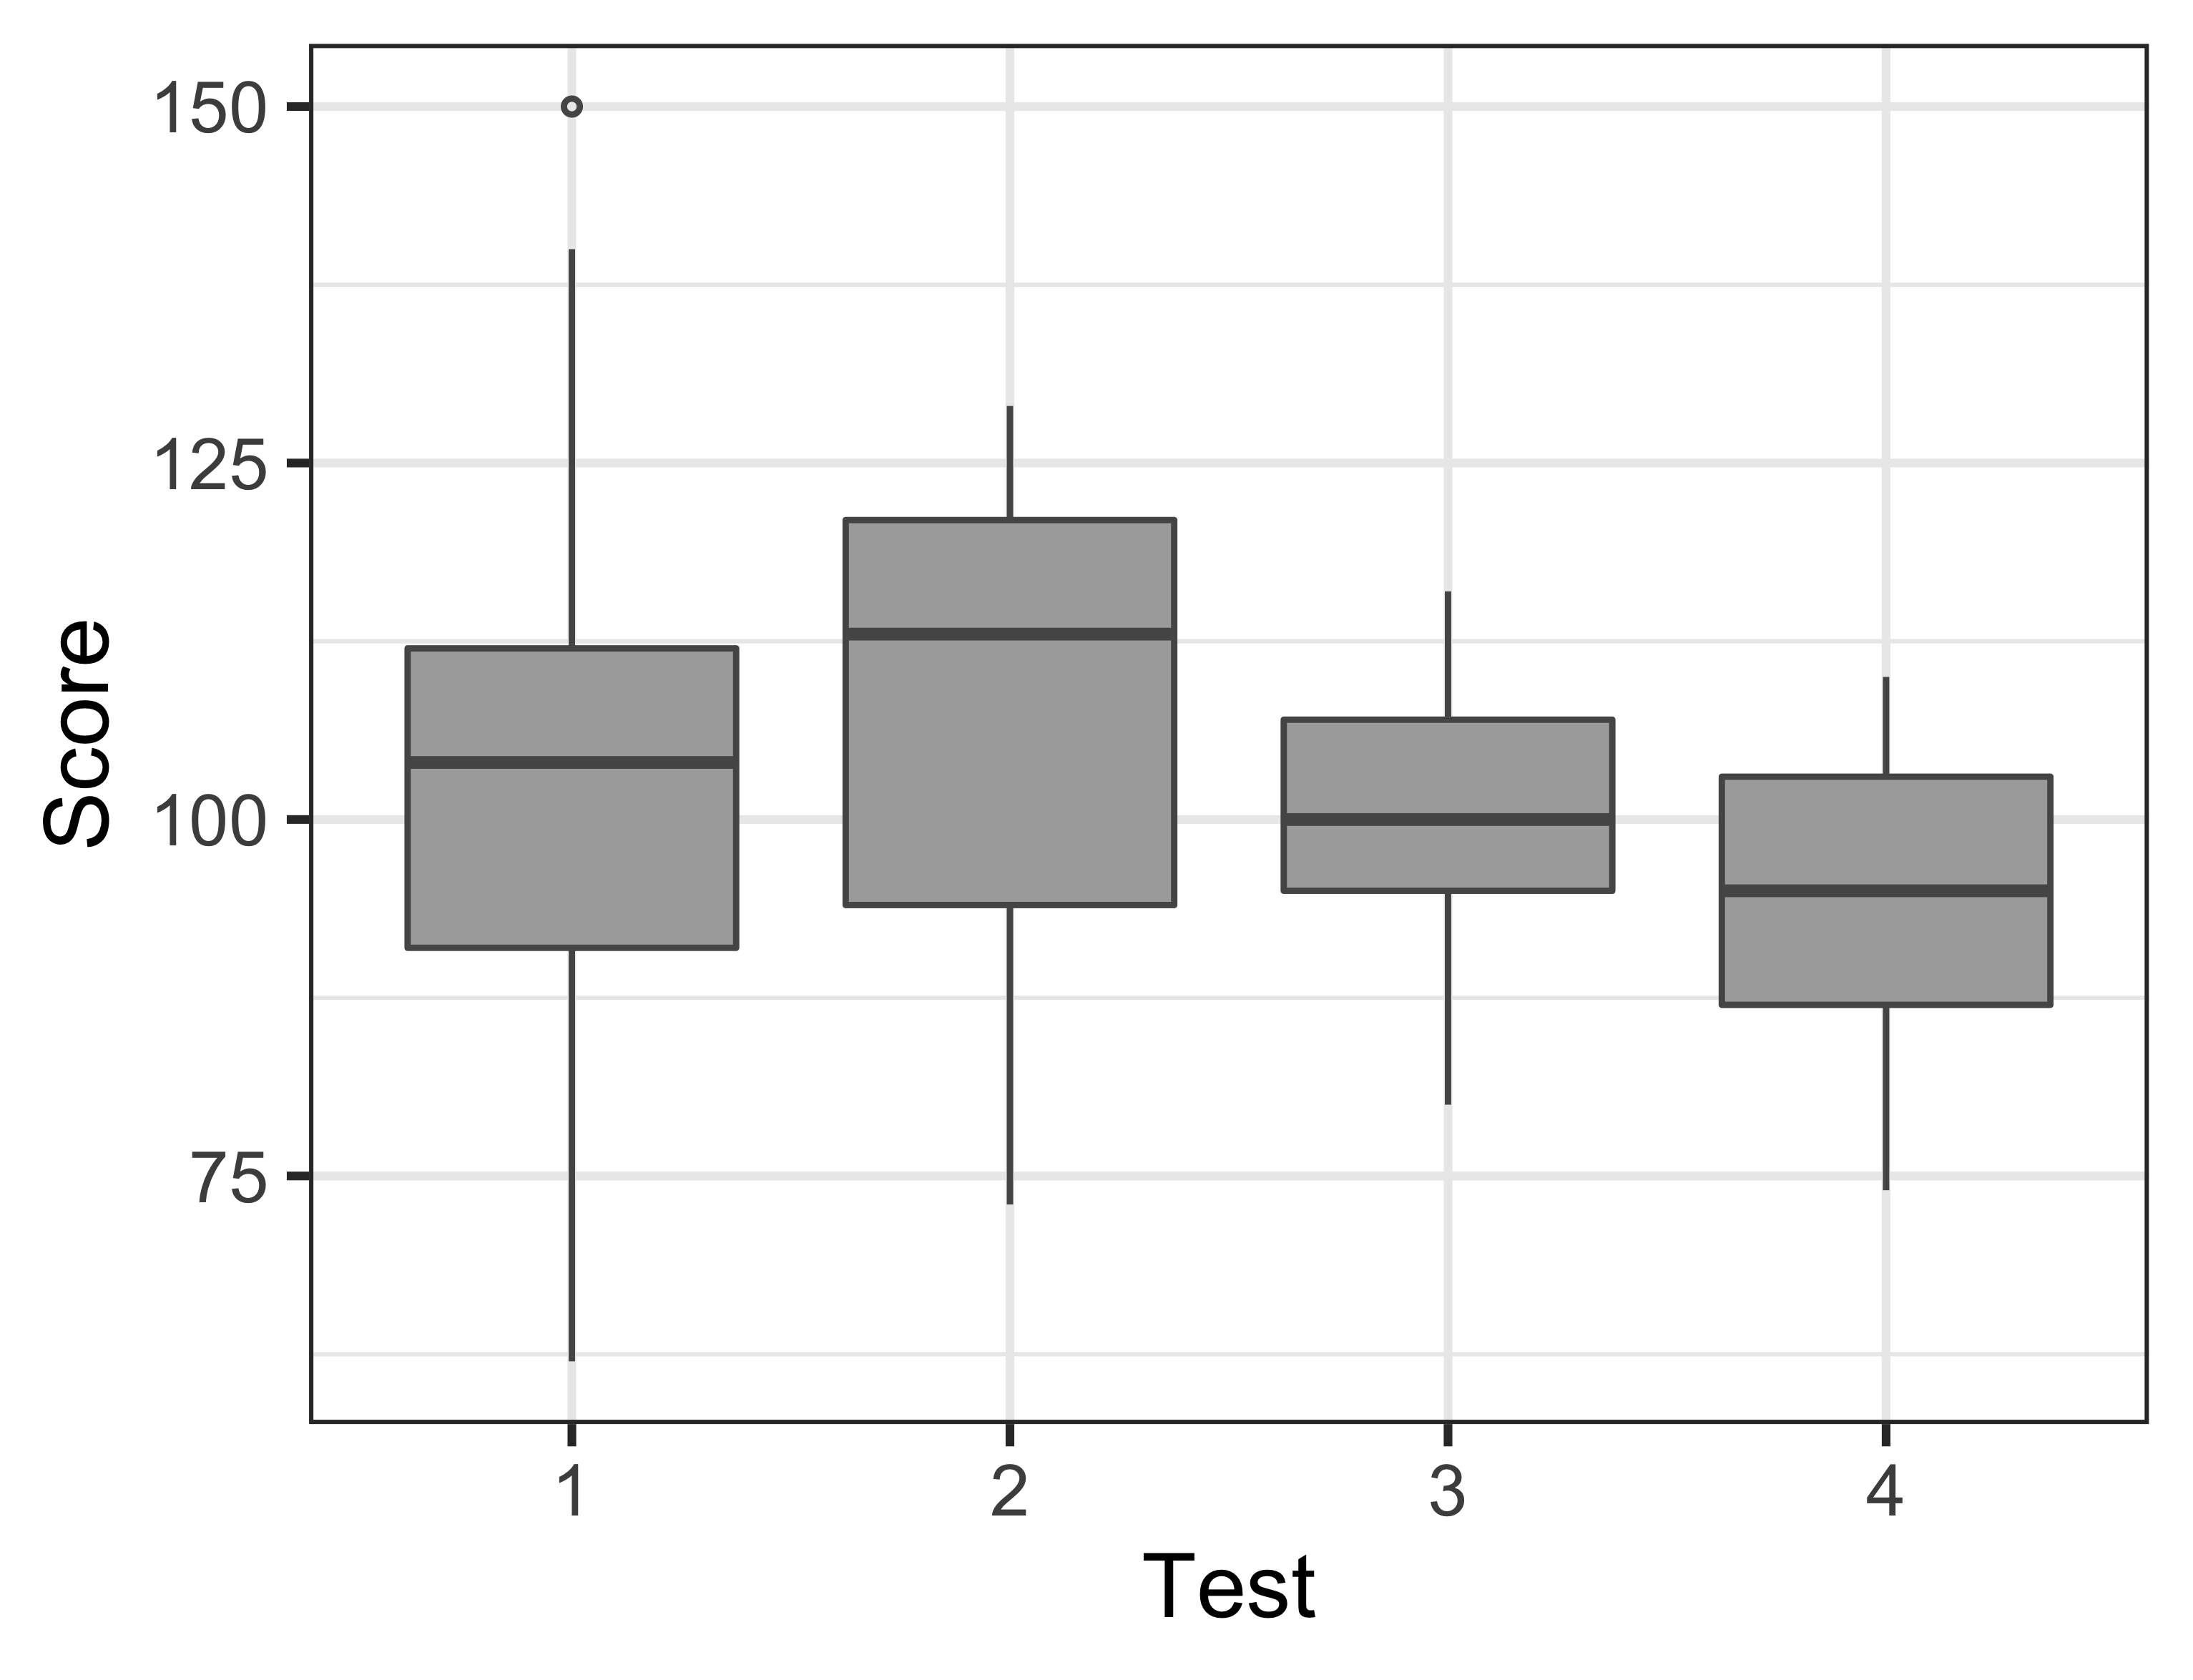
\includegraphics[width = 0.4\textwidth]{img/q03-boxplot.png}
        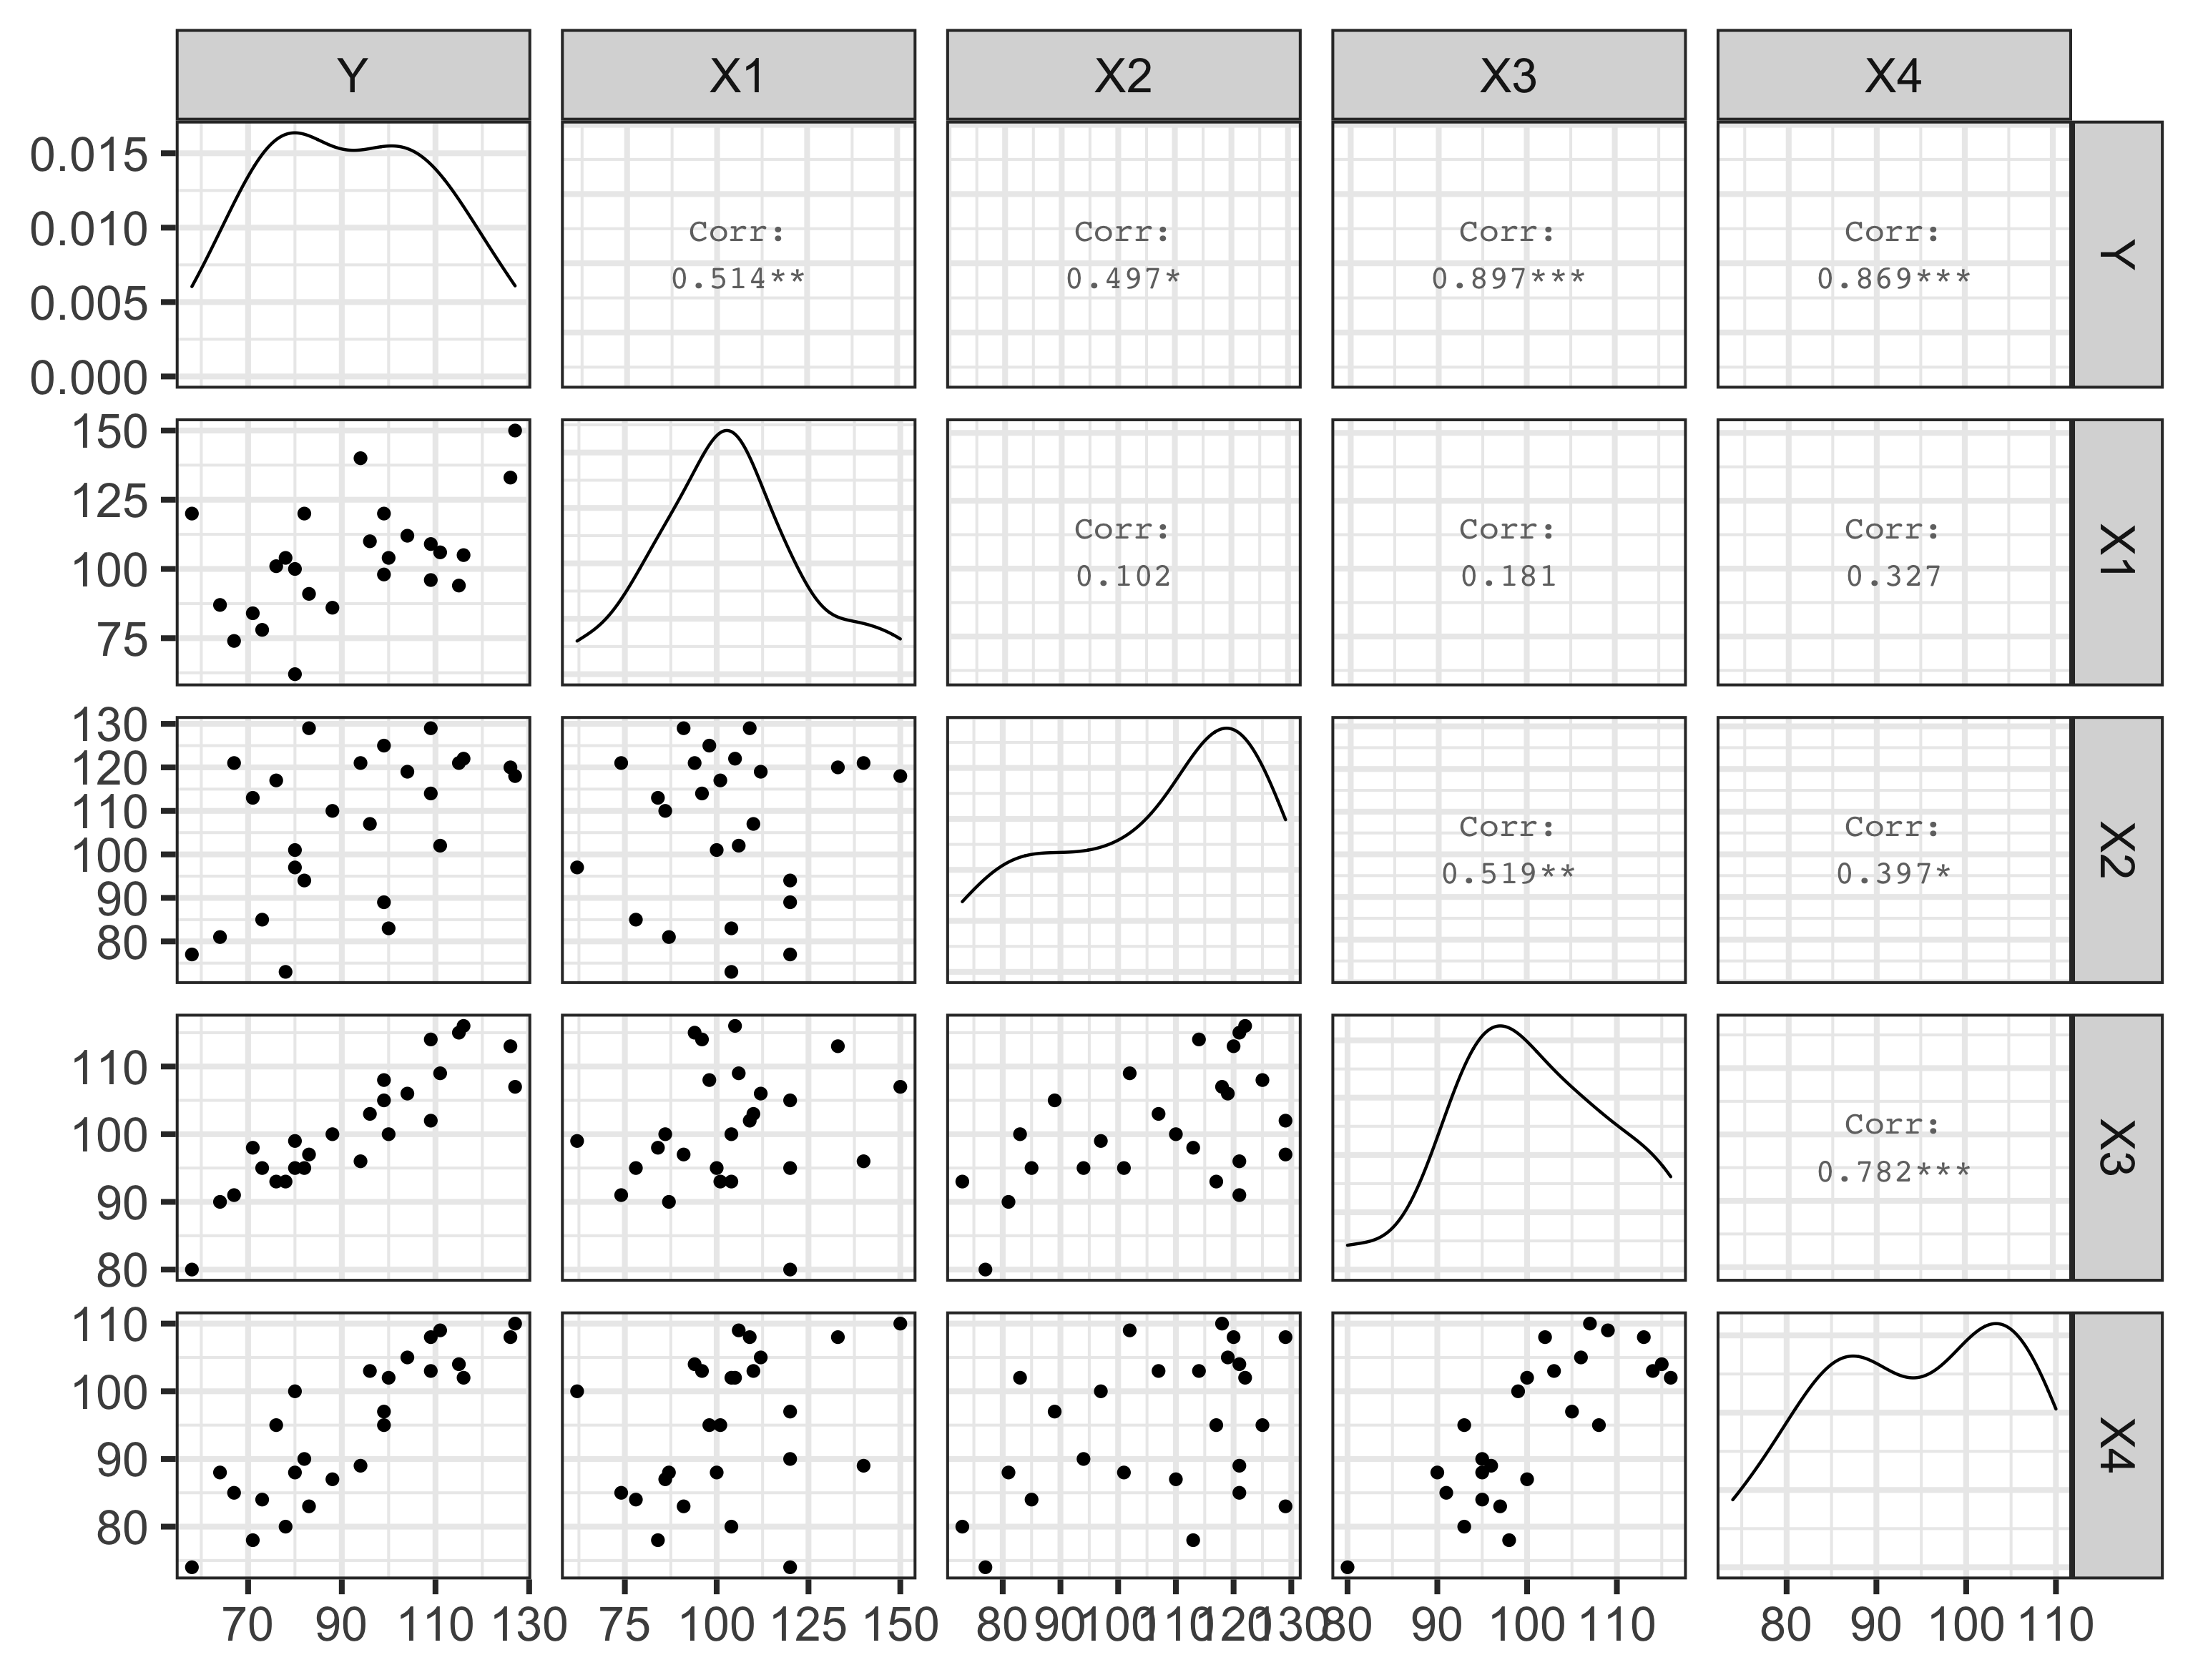
\includegraphics[width = 0.55\textwidth]{img/q03-correlation-matrix.png}
        \caption{Information about the test scores. }
        \label{q03-info}
    \end{figure}

    \item[(b)] The scatterplot matrix can be found in the right panel of Figure \ref{q03-info}. The only two variables that seem to have a strong correlation 
    with each other are tests 3 and 4, while tests 2 and 3 have somewhat of a correlation. We can also see that the job proficiency is highly-correlated with 
    tests 3 and 4. 

    \item[(c)] Letting \(Y\) be the job proficiency score and \(X_i\) be the \(i\)th test score for \(i = 1, \ldots, 4\), we fit the linear model 
    \(Y = \beta_0 + \beta_1 X_1 + \beta_2 X_2 + \beta_3 X_3 + \beta_4 X_4 + \epsilon\), where \(\mathbb{E}(\epsilon) = 0\) and \(\mathrm{Var}[\epsilon] = \sigma^2\).
    From the \texttt{R} output, the \(p\)-value for \(\beta_2\) is 0.404, meaning it is not significant. 
\end{itemize}

%' ============================================================================================================================================================
\section{Question 4} \noindent
\mycolaba{None}
\begin{itemize}
    \item[(a)] Using backward selection with AIC as the stopping criteria, our model includes tests 1, 3, and 4 as predictors, which is given by 
    \(\hat{Y} = -124.200 + 0.296 X_1 + 1.357 X_3 + 0.517 X_4 \). 
\end{itemize}

%' ============================================================================================================================================================
\section{Appendix A} \noindent

In this section, we will derive the result for \(m(\lambda)\), the log-likelikelihood as a function of only \(\lambda\).
Suppose we have our response vector \(\mathbf{y}\) and our observed data \(\mathbf{X} = \begin{bmatrix}
    \mathbf{1} & \mathbf{x}
\end{bmatrix}\). 
We are interested in fitting the model \(\mathbf{g}_{\lambda}(\mathbf{y}) = \mathbf{X}\bm{\beta} + \bm{\epsilon}\), where \(\mathbf{g}_{\lambda}(\mathbf{y})\)
is the transformed response vector (i.e. the \(i\)th element is given by \(g_{\lambda}(y_i)\)), \(\mathbb{E}[\bm{\epsilon}] = \mathbf{0}\), and 
\(\mathrm{Var}[\bm{\epsilon}] = \sigma^2 \mathbf{I}\). 
For notational ease, we will denote \(\mygfull\) as \(\myg\). 
If we make the further assumption that \(\bm{\epsilon}\) is normally distributed, i.e. 
\(\bm{\epsilon} \sim \mathrm{N}(\mathbf{0}, \sigma^2 \mathbf{I})\), then our response vector is also normally distributed, where
\(\myg \sim \mathrm{N}(\mathbf{X}\bm{\beta}, \sigma^2 \mathbf{I})\). It's density function (and thus it's likelihood function) is given by 
\begin{align*}
    % f(\myg \,|\, \mathbf{X}, \bm{\beta}, \sigma^2, \lambda)
    f(\myg \,|\, \bm{\beta}, \sigma^2, \lambda)
    % f(\myg)
    &= \frac{1}{\sqrt{\mathrm{det}(2 \pi \sigma^2 \mathbf{I})}} \cdot \mathrm{exp} \left( - \frac{(\myg - \mathbf{X}\bm{\beta})^T \big( \sigma^2 \mathbf{I} \big)^{-1} (\myg - \mathbf{X}\bm{\beta})}{2} \right) \\
    &= \frac{1}{(2\pi\sigma^2)^{n/2}} \cdot \mathrm{exp} \left( - \frac{(\myg - \mathbf{X}\bm{\beta})^T (\myg - \mathbf{X}\bm{\beta})}{2 \sigma^2} \right).
\end{align*}
Since \(\mathbf{y}\) is a transformation of \(\myg\) (via \(g_{\lambda}^{-1}\)), we can derive the density for \(\mathbf{y}\) as well. Notationally, this result may be somewhat 
confusing; even though we are finding the density for \(\mathbf{y}\), we will still express the density (partly) in terms of \(\myg\). It is important
to remember that \(\myg\) is a function of \(\mathbf{y}\). Because the \(i\)th element of \(\myg\) only depends on the \(i\)th element of \(\mathbf{y}\), the Jacobian
will be a diagonal matrix, and so 
\begin{align*}
    \mathbf{J}
    = \frac{\partial \myg}{\partial \mathbf{y}}
    = \mathrm{diag} \left( \frac{\partial g_{\lambda}(y_1)}{\partial y_1}, \ldots, \frac{\partial g_{\lambda}(y_n)}{\partial y_n} \right)
    = \mathrm{diag} \big( y_1^{\lambda - 1}, \ldots, y_n^{\lambda - 1} \big), 
\end{align*}
and so the density (and thus the likelihood) of \(\mathbf{y}\) is given by 
\begin{align*}
    g(\mathbf{y} \,|\, \bm{\beta}, \sigma^2, \lambda)
    = f \big( \myg(\mathbf{y}) \big) \cdot \big|\mathrm{det}(\mathbf{J})\big|
    = \frac{1}{(2\pi\sigma^2)^{n/2}} \cdot \mathrm{exp} \left( - \frac{(\myg - \mathbf{X}\bm{\beta})^T (\myg - \mathbf{X}\bm{\beta})}{2 \sigma^2} \right) \cdot \prod_{i=1}^n y_i^{\lambda - 1}.
\end{align*}
The log-likelihood \(\ell(\mathbf{y}) = \log g(\mathbf{y})\) is given by 
\begin{align*}
    \ell(\mathbf{y} \,|\, \bm{\beta}, \sigma^2, \lambda) 
    = - \frac{n}{2} \log (2\pi) - \frac{n}{2} \log (\sigma^2) - \frac{(\myg - \mathbf{X}\bm{\beta})^T (\myg - \mathbf{X}\bm{\beta})}{2 \sigma^2} + (\lambda - 1) \sum_{i=1}^n \log (y_i).
\end{align*}
As is standard with maximum likelihood estimation, we now differentiate \(\ell\) with respect to the unknown parameters, set the derivatives to zero, and solve to get the maximum value of \(\ell\). 
For now, we are going to leave \(\lambda\) fixed and differentiate with respect to \(\bm{\beta}\) and \(\sigma^2\). Doing this for both gives us 
\(\hat{\bm{\beta}}_{\mathrm{MLE}} = (\mathbf{X}^T\mathbf{X})^{-1}\mathbf{X}^T\myg\) and \(\hat{\sigma}^2_{\mathrm{MLE}} = \myg^T (\mathbf{I} - \mathbf{H}) \myg / n\), where 
\(\mathbf{H} = \mathbf{X}(\mathbf{X}^T\mathbf{X})^{-1}\mathbf{X}^T\) is the hat matrix. 
It is worth noting that both \(\hat{\bm{\beta}}_{\mathrm{MLE}}\) and \(\hat{\sigma}^2_{\mathrm{MLE}}\) are functions of \(\lambda\). 
Plugging these values back into \(\ell\) will maximize it with respect to \(\bm{\beta}\) and \(\sigma^2\), 
which means we will only have to maximize it with respect to \(\lambda\). 
With some simplification, our new loss function is 
\begin{align*}
    m(\lambda)
    \coloneqq \ell(\mathbf{y} \,|\, \hat{\bm{\beta}}_{\mathrm{MLE}}, \hat{\sigma}^2_{\mathrm{MLE}}, \lambda)
    % \triangleq \ell(\mathbf{y} \,|\, \hat{\bm{\beta}}_{\mathrm{MLE}}, \hat{\sigma}^2_{\mathrm{MLE}}, \lambda)
    = - \frac{n}{2} \log \left( \frac{2 \pi e}{n} \right) - \frac{n}{2} \log \big( \myg^T(\mathbf{I} - \mathbf{H}) \myg \big) + (\lambda - 1) \sum_{i=1}^n \log(y_i).
    % = - \frac{n}{2} \log \left( 2 \pi \mathrm{e} n \right) - \frac{n}{2} \log \big( \myg^T(\mathbf{I} - \mathbf{H}) \myg \big) + (\lambda - 1) \sum_{i=1}^n \log(y_i).
\end{align*}
Ideally, we would differentiate \(m\) with respect to \(\lambda\), set \(\partial m / \partial \lambda = 0\), and solve for \(\lambda\). I was unable to 
derive a closed form solution for the result, but it is still possible to use graphical techniques or numerical methods to find the optimal value of \(\lambda\). 

We recall that both \(\hat{\bm{\beta}}_{\mathrm{MLE}}\) and \(\hat{\sigma}^2_{\mathrm{MLE}}\) are functions of \(\lambda\), so we cannot know their value until \(\hat{\lambda}_{\mathrm{MLE}}\) has been determined.
Because of this, as we just showed, the likelihood function can be expressed as a function \(m(\lambda)\) that only depends on \(\lambda\), which can be maximized to find \(\hat{\lambda}_{\mathrm{MLE}}\). 
Once we find \(\hat{\lambda}_{\mathrm{MLE}}\), we can use this value to determine \(\hat{\bm{\beta}}_{\mathrm{MLE}}\) and \(\hat{\sigma}^2_{\mathrm{MLE}}\). 

% need to add info about transforming model back to y, here and in paragraph below
% maybe put into appendix?

%' ============================================================================================================================================================
\section{Appendix B} \noindent
Here we will derive the log-likelihood as a function of \(\theta\) and \(\bm{\lambda}\).
The methodology is identical to that of Appendix A, only now our response vector is \(\mygap{\mathbf{y}}\) and the data matrix is \(\gmat\). 
Using the exact same steps, we get our result \(m(\theta, \bm{\lambda})\).


%' ============================================================================================================================================================
\section{Appendix C} \noindent
Here is the correlation matrix for part (b) of question 2. 

\begin{figure}[ht]
    \centering
    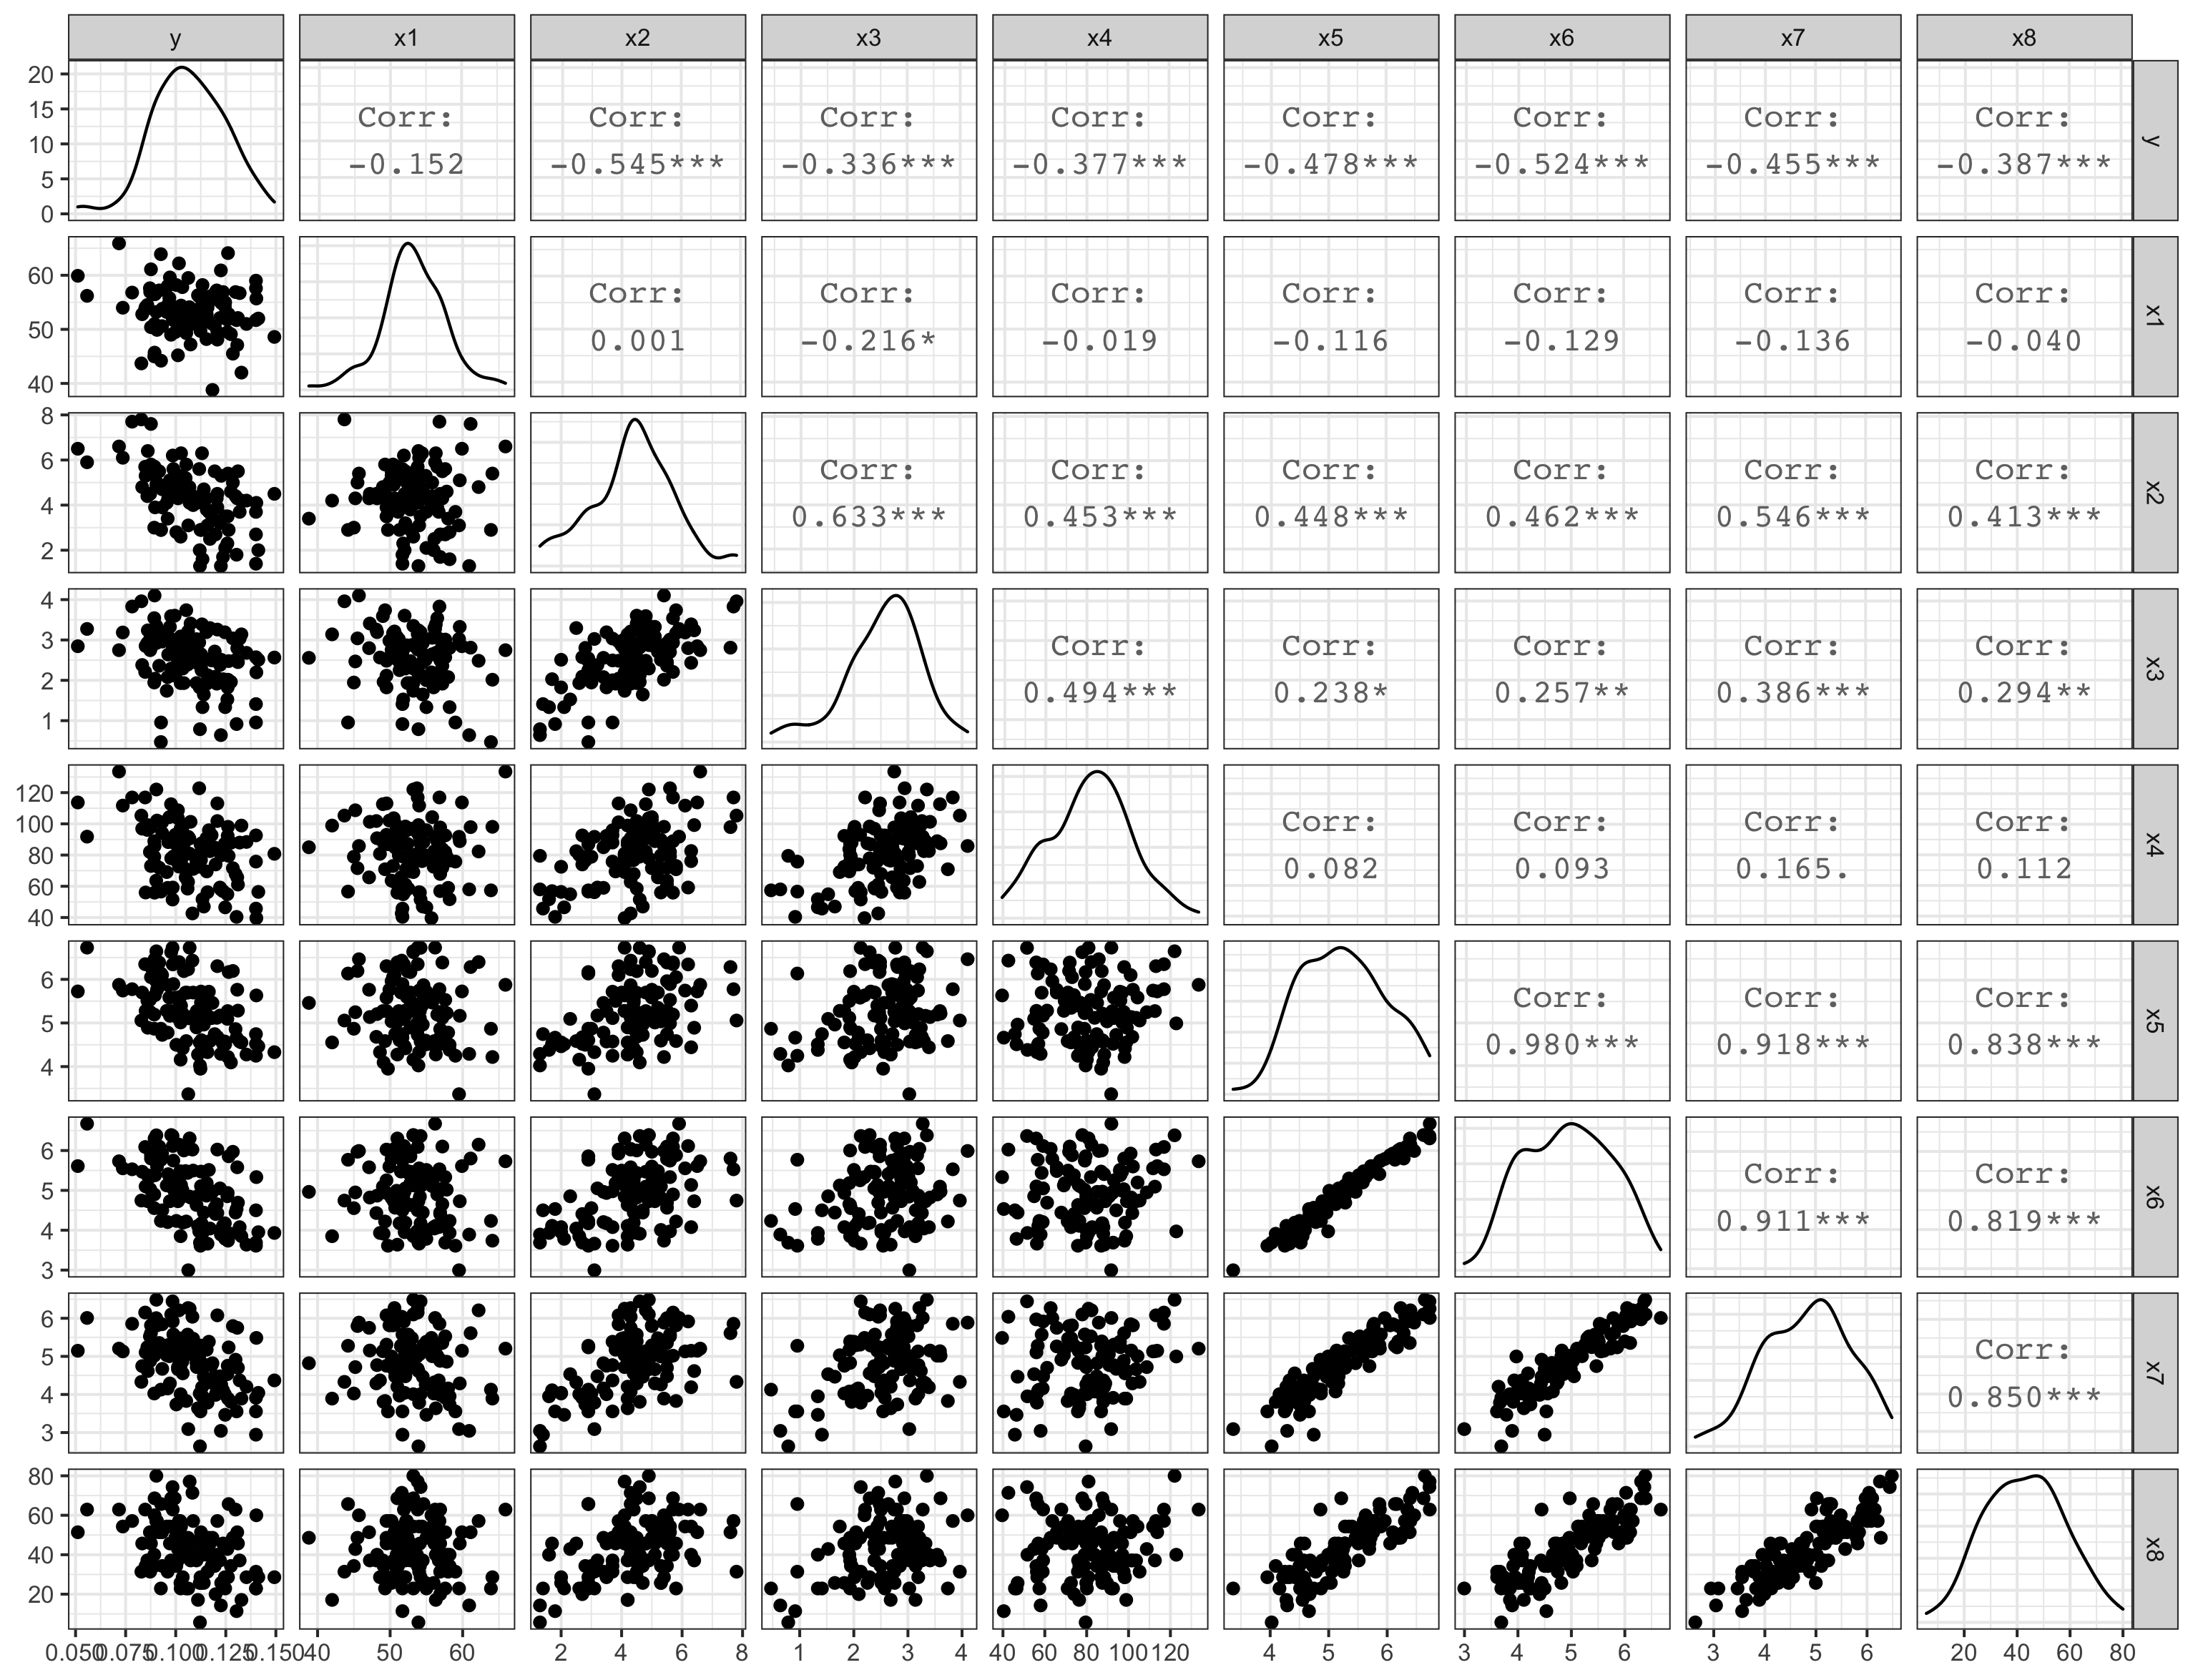
\includegraphics[width = \textwidth]{img/q02-correlation-matrix.png}
\end{figure}

\end{document}